% arara: pdflatex: { synctex: yes }
% arara: makeindex: { style: ctuthesis }
% arara: bibtex

% The class takes all the key=value arguments that \ctusetup does,
% and a couple more: draft and oneside
\documentclass[oneside]{ctuthesis}

\usepackage{siunitx}
\usepackage{nomencl}
\usepackage{setspace}
\usepackage{indentfirst}

%%%%%%%%%%%%%%%%%% insert images from other directory
\usepackage{graphicx}
\graphicspath{{./images/}}

%%%%%%%%%%%%%%%%%%%%%%%%%%%%%%%%%%%%%% this shit is here to break long url into more lines
\usepackage{url}
\makeatletter
\g@addto@macro{\UrlBreaks}{\UrlOrds}
%\makeatother

%%%%%%%%%%%%%%%%%%%%%%%%%%%%%%%%%%%%%% this shit is here to prevent breaking words on the edge of a line
\tolerance=1
\emergencystretch=\maxdimen
\hyphenpenalty=10000
\hbadness=10000



%%%%%%%%%%%%%%%%%%%%%%%%%%.this makes the differed text make different
%DIF PREAMBLE EXTENSION ADDED BY LATEXDIFF
%DIF UNDERLINE PREAMBLE %DIF PREAMBLE
\RequirePackage[normalem]{ulem} %DIF PREAMBLE
\RequirePackage{color}\definecolor{RED}{rgb}{1,0,0}\definecolor{BLUE}{rgb}{0,0,1} %DIF PREAMBLE
\providecommand{\DIFadd}[1]{{\protect\color{blue}\uwave{#1}}} %DIF PREAMBLE
\providecommand{\DIFdel}[1]{{\protect\color{red}\sout{#1}}}                      %DIF PREAMBLE
%DIF SAFE PREAMBLE %DIF PREAMBLE
\providecommand{\DIFaddbegin}{} %DIF PREAMBLE
\providecommand{\DIFaddend}{} %DIF PREAMBLE
\providecommand{\DIFdelbegin}{} %DIF PREAMBLE
\providecommand{\DIFdelend}{} %DIF PREAMBLE
%DIF FLOATSAFE PREAMBLE %DIF PREAMBLE
\providecommand{\DIFaddFL}[1]{\DIFadd{#1}} %DIF PREAMBLE
\providecommand{\DIFdelFL}[1]{\DIFdel{#1}} %DIF PREAMBLE
\providecommand{\DIFaddbeginFL}{} %DIF PREAMBLE
\providecommand{\DIFaddendFL}{} %DIF PREAMBLE
\providecommand{\DIFdelbeginFL}{} %DIF PREAMBLE
\providecommand{\DIFdelendFL}{} %DIF PREAMBLE
%DIF END PREAMBLE EXTENSION ADDED BY LATEXDIFF


% to print code
\usepackage{listings}
\usepackage{color}
\definecolor{dkgreen}{rgb}{0,0.6,0}
\definecolor{gray}{rgb}{0.5,0.5,0.5}
\definecolor{mauve}{rgb}{0.58,0,0.82}
\lstset{frame=tb,
  language=C++,
  aboveskip=3mm,
  belowskip=3mm,
  showstringspaces=false,
  columns=flexible,
  basicstyle={\small\ttfamily},
  numbers=none, 
  % numberstyle=\tiny\color{gray},
  % keywordstyle=\color{blue},
  % commentstyle=\color{dkgreen},
  % stringstyle=\color{mauve},
  breaklines=true,
  breakatwhitespace=true,
  tabsize=3
}
% to display source code
\definecolor{mGreen}{rgb}{0,0.6,0}
\definecolor{mGray}{rgb}{0.5,0.5,0.5}
\definecolor{mPurple}{rgb}{0.58,0,0.82}
\definecolor{backgroundColour}{rgb}{0.95,0.95,0.92}
\lstdefinestyle{CStyle}{
    backgroundcolor=\color{backgroundColour},   
    commentstyle=\color{mGreen},
    keywordstyle=\color{magenta},
    numberstyle=\tiny\color{mGray},
    stringstyle=\color{mPurple},
    basicstyle=\footnotesize,
    breakatwhitespace=false,         
    breaklines=true,                 
    captionpos=b,                    
    keepspaces=true,                 
    numbers=left,                    
    numbersep=5pt,                  
    showspaces=false,                
    showstringspaces=false,
    showtabs=false,                  
    tabsize=2,
    language=C
}
\lstdefinestyle{log}{
    backgroundcolor=\color{backgroundColour},   
    % commentstyle=\color{mGreen},
    % keywordstyle=\color{magenta},
    % numberstyle=\tiny\color{mGray},
    % stringstyle=\color{mPurple},
    basicstyle=\footnotesize,
    breakatwhitespace=false,         
    breaklines=true,                 
    % captionpos=b,                    
    keepspaces=true,                 
    numbers=none,                    
    numbersep=5pt,                  
    showspaces=false,                
    showstringspaces=false,
    showtabs=false,                  
    tabsize=2,
    language=C
}


%%%
% \usepackage{framed}
% \usepackage{hyperref}
% % \usepackage[czech]{babel}
% \usepackage[utf8]{inputenc}
% \usepackage[T1]{fontenc}

\usepackage{dirtree}        %directory tree visualisation
\usepackage{blindtext}
\parskip=12pt % adds vertical space between paragraphs

\usepackage{xcolor}
\definecolor{shadecolor}{RGB}{230,230,230}

% to print code
\usepackage{listings}
\usepackage{color}
%%%

\ctusetup{
%	preprint = \ctuverlog,```%%%%%%%%%%%%%%%%%%%%%%%%% toto je cislo na kazde strance dole ktere tam nema byt
%	mainlanguage = english,
%	titlelanguage = english,
	mainlanguage = czech,
	otherlanguages = {czech},
	% title-czech = {Low power wireless sensor network},
	title-czech = {Bezdrátová senzorová síť pro přístupový systém},
	title-english = {Wireless sensor network for access control system},
	subtitle-czech = {},
	subtitle-english = {},
	faculty = F3,
	department-czech = {Katedra telekomunikační techniky},
	department-english = {Department of Telecommunications Engineering},
	author = {Tomáš Hyhlík},
	supervisor = {Ing. Bc. Marek Neruda, Ph.D},
	supervisor-address = {},
	supervisor-specialist = {Ing. Bc. Lukáš Vojtěch, Ph.D},
	fieldofstudy-english = {Electronics and Communications},
	subfieldofstudy-english = {Electronics},
	fieldofstudy-czech = {Elektronika a komunikace},
	subfieldofstudy-czech = {Elektronika},
	keywords-czech = {Access control system, LoRa, LPWAN, WSN.},
	keywords-english = {Access control system, LoRa, LPWAN, WSN.},
	day = 12,
	month = 10,
	year = 2019,
	specification-file = {zav_prace.pdf},
%	front-specification = true,
%	front-list-of-figures = false,
%	front-list-of-tables = false,
%	monochrome = true,
%	layout-short = true,
}

\ctuprocess

\addto\ctucaptionsczech{%
	\def\supervisorname{Vedoucí}%
	\def\subfieldofstudyname{Studijní program}%
}

\ctutemplateset{maketitle twocolumn default}{
	\begin{twocolumnfrontmatterpage}
		% \ctutemplate{twocolumn.thanks}
		% \ctutemplate{twocolumn.declaration}
		\ctutemplate{twocolumn.abstract.in.titlelanguage}
		\ctutemplate{twocolumn.abstract.in.secondlanguage}	
		\ctutemplate{twocolumn.tableofcontents}
		\ctutemplate{twocolumn.listoffigures}
	\end{twocolumnfrontmatterpage}
}

% Theorem declarations, this is the reasonable default, anybody can do what they wish.
% If you prefer theorems in italics rather than slanted, use \theoremstyle{plainit}
\theoremstyle{plain}
\newtheorem{theorem}{Theorem}[chapter]
\newtheorem{corollary}[theorem]{Corollary}
\newtheorem{lemma}[theorem]{Lemma}
\newtheorem{proposition}[theorem]{Proposition}

\theoremstyle{definition}
\newtheorem{definition}[theorem]{Definition}
\newtheorem{example}[theorem]{Example}
\newtheorem{conjecture}[theorem]{Conjecture}

\theoremstyle{note}
\newtheorem*{remark*}{Remark}
\newtheorem{remark}[theorem]{Remark}

\setlength{\parskip}{5ex plus 0.2ex minus 0.2ex}

% Abstract in Czech
\begin{abstract-czech}
	todo
	% The Wireless Sensor Network (WSN) plays an important role in the Internet of Things (IoT). 
	% It is very suitable for intelligent buildings providing a convenient way to collect sensor data and control electronic devices in the building and its surroundings.
	% %Nowadays, existing intelligent buildings include some electronic systems, such as access control systems. 
	% %As the WSN becomes neccesary, the effort of imlementation of WSN into existing smart buildings grow.
	% %It may be easier and cheaper to extend an existing electronic system with WSN instead of integrating an entire new WSN system into the building.
	% This paper proposes an extension of the existing access control system with WSN. Design of sensor nodes and gateway connected to the existing RS485 network is performed. The results of a long-term operation measurement in one university floor show the maximum number of sensor nodes simultaneously transmitting data in RS485 network is up to hundreds or thousands in dependence on used RS485 data rate and used reserve of data rate which prevent from malfunction of the access control system. The results prove the WSN can be effectively used in an existing RS485 infrastructure. 
\end{abstract-czech}

% Abstract in English
\begin{abstract-english}
	% The Wireless Sensor Network (WSN) plays an important role in the Internet of Things (IoT). 
	% It is very suitable for intelligent buildings providing a convenient way to collect sensor data and control electronic devices in the building and its surroundings.
	% %Nowadays, existing intelligent buildings include some electronic systems, such as access control systems. 
	% %As the WSN becomes neccesary, the effort of imlementation of WSN into existing smart buildings grow.
	% %It may be easier and cheaper to extend an existing electronic system with WSN instead of integrating an entire new WSN system into the building.
	% This paper proposes an extension of the existing access control system with WSN. Design of sensor nodes and gateway connected to the existing RS485 network is performed. The results of a long-term operation measurement in one university floor show the maximum number of sensor nodes simultaneously transmitting data in RS485 network is up to hundreds or thousands in dependence on used RS485 data rate and used reserve of data rate which prevent from malfunction of the access control system. The results prove the WSN can be effectively used in an existing RS485 infrastructure. 
\end{abstract-english}

% % Acknowledgements / Podekovani
% \begin{thanks}
% I would like to thank Supervisor Ing. Bc. Marek Neruda Ph.D and Supervisor-specialist Ing. Bc. Lukáš Vojtěch Ph.D for helping me with this project. Also I would like to thank IMA s.r.o. company, which helped me to get compatible cards to the HID Prox Point plus reader, which is used for the second system design.
% \end{thanks}


% % Declaration / Prohlaseni
% \begin{declaration}
% I declare that I have developed the presented work independently and that I have
% listed all information sources used in accordance with the Methodical Guidelines on
% Maintaining Ethical Principles During the Preparation of Higher Education Theses.

% In Prague, \ctufield{day}.~\monthinlanguage{title}~\ctufield{year}
% \end{declaration}

% Only for testing purposes
\listfiles
\usepackage[pagewise]{lineno}
\usepackage{lipsum,blindtext}
\usepackage{mathrsfs} % provides \mathscr used in the ridiculous examples

\newcommand{\abbrlabel}[1]{\makebox[3cm][l]{\textbf{#1}\ \dotfill}}
\newenvironment{abbreviations}{\begin{list}{}{\renewcommand{\makelabel}{\abbrlabel}}}{\end{list}}


%%%%%%%%%%%%%%%%%%%%%%%%%%%%%%%%%  BEGIN %%%%%%%%%%%%%%%%%%%%%%%%%%%%%%%%%%%%%%%%%
\begin{document}

\maketitle

% \ctutemplate{specification.as.chapter}       % ZADANI

%\rule{\linewidth}{1pt}     % this shit was here for the url cut
\titlespacing*{\chapter}					{0pt}	{0ex}{0ex}
\titlespacing*{\section} 					{0pt}	{0ex}{-3ex}
\titlespacing*{\subsection} 			{0pt}	{0ex}{-3ex}
\titlespacing*{\subsubsection}		 {0pt}	{0ex}{-4ex}
\titlespacing*{\paragraph} 			{0pt}	{0ex}{-4ex}
\titlespacing*{\aubparagraph} 		{0pt}	{0ex}{-4ex}

% \section{List of Abbreviations}
\section{Seznam zkratek}
\begin{abbreviations}
	\item[AES]		Advanced Encryption Standard 
	\item[AI]		Artifical Inteligence
	\item[AppSKey]	Application Session Key	
	\item[ASCII] 	American Standard Code for Information Interchange
	\item[BLE]		Bluetooth Low Energy 
	\item[CMAC]		Cipher-based message authentication code 
	\item[CMSIS]	Cortex Microcontroller Software Interface Standard  
	\item[CPU]		Central Processing Unit
	\item[CR] 		Carriage Return
	\item[CRC] 		Cyclic Redundancy Check
	\item[EEPROM] 	Electrically Erasable Programmable Read-Only Memory
	\item[FIFO]		First In First Out 
	\item[GPIO]		General Purpose Input Output 
	\item[HAL]		Hardware Abstraction Layer 
	\item[HW]		HardWare
	\item[IDE]		Integrated Development Environment 
	\item[IoT] 		Internet of Things
	\item[ISM]		Industrial, scientific and medical 
	\item[IWDG]		Independent Watchdog 
	\item[LAN]		Local Area Network
	\item[LBT]		Listen Before Talk 
	\item[LF]		Line Feed 
	\item[LPWAN]   	Low Power Wide Area Network 
	\item[LPWSN] 	Low Power Wireless Sensor Network	
	\item[MCU] 		Micro Controller Unit
	\item[NwkSKey]	Network Session Key
	\item[PC]		Personal Computer 
	\item[PCB]		Printed Circuit Board 
	\item[RF]		Radio Frequency
	\item[RTOS]		Real Time Operating System 
	% \item[I2C]   	Inter-integrated Circuit
	% \item[IPv6] 	Internet Protocol version 6

	% \item[M2M]		machine to machine
	% \item[RPMA]		Random Phase Multiple Access
	\item[SDK]	 	Software development kit
	\item[SF]		Spreading Factor
	\item[SPI]   	Serial Peripheral Interface 
	\item[UART]		Universal Asynchronous Receiver Transmitter 
	\item[USB]		Universal Serial Bus 
	\item[WSN]		Wireless Sensor Network

\end{abbreviations}

%%%%%%%%%%%%%%%%%%%%%%%%%%%%%%%%%%%%%%%%%%%%%%%%
% \chapter{The purpose of low power wireless sensor networks and its state of art}
\chapter{Úvod}
Se stále rostoucím využitím IoT (Internet of Things) aplikací v různých oblastech, např. zemědělství, smart metering, smart cities, smart homes, roste i počet dostupných bezdrátových technologií se zaměřením na 
nízkou spotřebu energie, velký dosah, nízkou přenosovou rychlost a nízkou cenu.

IoT aplikace vyžadující krátký dosah, jako je použití v domácnostech (smart home) většinou využívají bezdrátové technologie Zigbee nebo Bluetooth, tedy technologie používající pásmo ISM (Industrial Scientific and Medical) 2.4 GHz \cite{Design and Implementation of an IoT Assisted Real Time ZigBee Mesh WSN}, \cite{Internet of Things (IoT) for building Smart Home System}.
IoT aplikace vyžadující dlouhý dosah jsou vetšinou založené na druhu technologií LPWAN (Low Power Wide Area Network) \cite{A comparative study of LPWAN technologies for large-scale IoTdeployment}. 

Many LPWAN wireless communication technologies appeared during its evolution with unlicensed ISM band, e.g., LoRa and SigFox and licensed band, e.g., NarrowBand-Internet of Things (NB-IoT) and Long Term Evolution-Machine Type Communication (LTE-M).
% The LPWAN technologies aim to have range up to 10–15 km in rural areas and 2–5 km in urban areas \cite{Long-Range Communications in Unlicensed Bands} and can have one of the following topologies: star (centralized), star of stars (decentralized) and mesh (distributed) \cite{high density LPWAN}.
% Very low power consumption should allow sensor nodes a very long battery life, even greater than 10 years.
% The low cost of hardware (HW) is achieved by fully integrated transceivers and minimized number of off-chip components \cite{MURS Band for LPWAN Applications}.

% The industry of IoT is growing because of its enormous potential.
% Cisco study \cite{IoT cisco study} says IoT will be combined with other technologies such as artificial inteligence (AI), fog computing and blockchain. Such a combination of technologies will provide greater value of investment for companies. 
% IoT applications in smart cities require a scalable network coverage. This can be achieved by interconnection of multiple gateways as proposed in \cite{Flexible Wireless Sensor Network for smart lighting applications}, where all gateways are connected to web server accessible via the Internet. It aims to manage urban street lighting and the implementation of smart metering is also considered as a future work.
% Similar application is proposed in paper \cite{Design and Implementation of an IoT Assisted Real Time ZigBee Mesh WSN} which focuses on assisted real-time automatic meter reading (AMR) in cities, but the scalable range is established by mesh network topology.
% The IoT applications in a smart buildings concept can be proposed as shown in
% \cite{Internet of Things (IoT) for building Smart Home System}, where nodes exchange data with the cloud via a Wi-Fi router or Bluetooth gateway connected to the Internet. 
% Similar application is proposed in \cite{Building a Smart Home System with WSN and Service Robot} where nodes are controlled by a master node via Zigbee network that is conncected to a PC via RS232.
% Basic smart metering systems can be proposed with a gateway connected to a PC where the data are processed as proposed in \cite{A Meter Reading System Based on WSN}, \cite{Smart Water Meter System for User-Centric Consumption Measurement} and \cite{Radio Data Infrastructure for Remote Monitoring}.
% A long-range metering system can be established by multiple gateways connected to a network server from which data are obtained by the application server \cite{Smart Electric Meter Using LoRA Protocols and Iot applications}. 
% % Such network andrchitecture also uses The Things Network (TTN) \cite{ttn} which is open LoRaWAN network available for anyone to use by connecting his own nodes and to contribute by connecting his own gateway.
% Similar network is proposed in Smart Farm application \cite{Implement Smart Farm with IoT Technology} with the difference that nodes can also be connected to the gateway via RS485 which forms a hybrid wired /wireless system.

% This paper proposes to extend the access control system to include a low power Wireless Sensor Network (WSN) which can be used for smart metering applications, smart building applications and the building surroundings which is related to smart city applications. 
% The WSN gateway is connected by the same way as a card reader is connected in the access control system, therefore it also has to support the same protocol. This can lead to complications since the reader is ment to transmit a short packets with user ID when the user's credential is attached to it. 
% The WSN gateway is designed and tested in access control system of one university floor. The results show the infrastructure of access control system can manage up to thousands sensor nodes in dependence on used RS485 data rate. 


%%%%%%%%%%%%%%%%%%%%%%%%%%%%%%%%%%%%%%%%%%%%%%%%%%%%%%%%%%%%%%%%%%%%%%%%%%%%%%%%%%%%%%%
%       NOT USED
%%%%%%%%%%%%%%%%%%%%%%%%%%%%%%%%%%%%%%%%%%%%%%%%%%%%%%%%%%%%%%%%%%%%%%%%%%%%%%%%%%%%%%%

% \cite{Implement Smart Farm with IoT Technology} includes design of hybrid (wired / wireless) smart metering system for multiple farms with multiple LPWAN gateways where nodes are sensors and actuators and communicate via MQTT. As the future work there is said that it can also be used for monitoring grazing livestock by attachin nodes to its bodies and also the system is supposed to be used for studying the development of environmental algorithms for optimization of plants growth with use of environmental data and plant growth data.
% https://ieeexplore.ieee.org/stamp/stamp.jsp?tp=&arnumber=8323908

%%%%%%%%%%%%%%%%%%%%%%%%%%%%%%%%%%%%%%%%%%%%%%%%%%%%%%%%%%%%%%%%%%%%%%%
% not used articles:
% Article \cite{ZigBee-based Vehicle Access Control System} icludes design of vehicle access control system based on Zigbee network which is connected through network coodrinator via RS232 to PC.
% https://ieeexplore.ieee.org/stamp/stamp.jsp?tp=&arnumber=5453569






%%%%%%%%%%%%%%%%%%%%%%%%
\part{Theoretical part}
									
\chapter{Přístupové systémy}
  \chapter{Výběr bezdrátové technologue pro senzorovou síť}
Navržená senzorová síť je napojena na infrastrukturu zavedeného přístupového systému v budově zákazníka s dosahem po celé budově a jejím okolí. Takto navržená síť umožní v těchto prostorách snímání dat z desítek senzorů.
Mezi hlavní kritéria pro vybranou bezdrátovou technologii patří nízká spotřeba energie koncových zařízení, nízká cena, jednoduchost implementace a možnost připojení koncových zařízení třetích stran.
Pro jednoduchost implementace vybraná bezdrátová technologie tedy musí používat pouze bezlicenční pásmo ISM a musí umožňovat uplementaci celé sítě bez závislosti na siti třetích stran. 

\section{Kandidátní bezdrátové technlogie}
Níže jsou popsány dostupné bezdrátové technologie vyhovující stanoveným kritériím pro tento projekt.

\subsection{IQRF}
IQRF je technologie vyvinuta IQRF aliancí \cite{iqrf_alliance}, která je jediným výrobcem IQRF transceiveru \cite{iqrf_transceivers} za cenu v rozsahu \$15-20 za kus a k tomu poskytuje nástroje jako je SDK \cite{iqrf_sdk} a IDE \cite{iqrf_ide}.
Technologie IQRF bývá použita k realizaci sítí o topologii typu mesh nebo hvězdice.
Jedna síť má jednoho koordinátora, který slouží jako gateway a může obsahovat až 240 zařízení (včetně koordinátora). Pro požadavek vyššího počtu zařízení je efektivnější zřetězit více sítí, s jednotlivými koordinátory a různými RF kanály pro vyšší propustnost.
% https://iqrf.org/support/networkingfaq
Dosah na přímou viditelnost je až 500 m a velikost payloadu jednoho packetu může být až 64 B.
Z hlediska kriérií pro tento projekt je u této technologie nevýhodou nízký počet zařízení třetích stran dostupných na trhu. 
Většinou je tato technologie použita pro realizaci uživatelsé sítě, kde gateway je použita jedna z dostupných od IQRF aliance a koncová zařízení sítě jsou vytvořena vývojáři s použitím transceiverů od IQRF aliance
\cite{paper_iqrf}.


\subsection{Wireless M-Bus}
Wireless M-Bus (Meter-Bus) je standard specifikovaný v evropské normě EN 13757, popisující fyzickou, síťovou a aplikační vrstvu, původně navržen pro aplikace bezdrátového měření jako rozšíření průmyslové datové sběrnice M-Bus \cite{wirelessMBus_automatizace}.
Po několika letech v průmyslu bezdrátových měřících systémů se tato technologie rozšířila do oblasti průmyslu senzorových sítí.
Komunikace koncových zařízení je rozdělena do několika módů v závislosti na orientaci komunikace a objemu vysílaných dat \cite{wirelessMBus01} \cite{wirelessMBus02}. 
Wireless M-Bus síť má hvězdicovou topologii o dosahu 500 m v pásmu 868 MHz.
Komunikaci vždy zahajuje koncové zařízení, které koncentrátor obsluhuje.
Transceivery vyrábí více různých firem za cenu okolo \$25-30 za kus.


\subsection{LoRa}
LoRa (Long Range) je modulace navržena firmou Semtech, LoRa Alliance vytvořila síťový protokol s názvem LoRaWAN postaven na fyzické vrstvě LoRa.
Síť má hvězdicovou topologii, kde komunikaci zahajuje koncové zařízení a koncentrátor ho obsluhuje.
Pro nízkou spotřebu protokol umožňuje ladit SF (Spreading Factor) neboli přenosovou rychlost, pro regulaci dosahu, který je až 15-22 km mimo městskou část a 3-8 km ve městské části \cite{lorawan_specification}.
V některých oblastech některé firmy poskytují pokrytí LoRaWAN sítí a proto je tato technologie velmi populární, Na trhu je mnoho koncových zařízení i gatewayí, s jejichž vzájemnou kompatibilitou neni problém. Gateway přeposílá přijaté packety s daty z koncových zařízení na server, kde je payload zpracován na základě dokumentace od výrobce daného koncového zařízení.
Semtech je jediným výrobcem integrovaných obvodů podporujících LoRa modulaci. Na trhu je dostupných mnoho transceiverů, které používají tento integrovaný obvod, některé dokonce obsahují implementovaný LoRaWAN stack.
Transceiver pro gateway má cenu okolo \$130 a umožňuje současně přijímat packety od koncových zařízení na více kanálech a přenosových rychlostech. Je zde i možnost udělat jednokanálovou gateway, která je schopna přijímat v jednu chvíli pouze jednom kanále a jedné přenosové rychlosti s použitím transceiveru pro koncová zařízení za cenu okolo \$5-20. V takové sítí pak musí být všechna koncová zařízení nakonfigurována na jednu konkrétní frekvenci a přenosovou rychlost.


% \begin{figure}[!h]
%     \centering
%     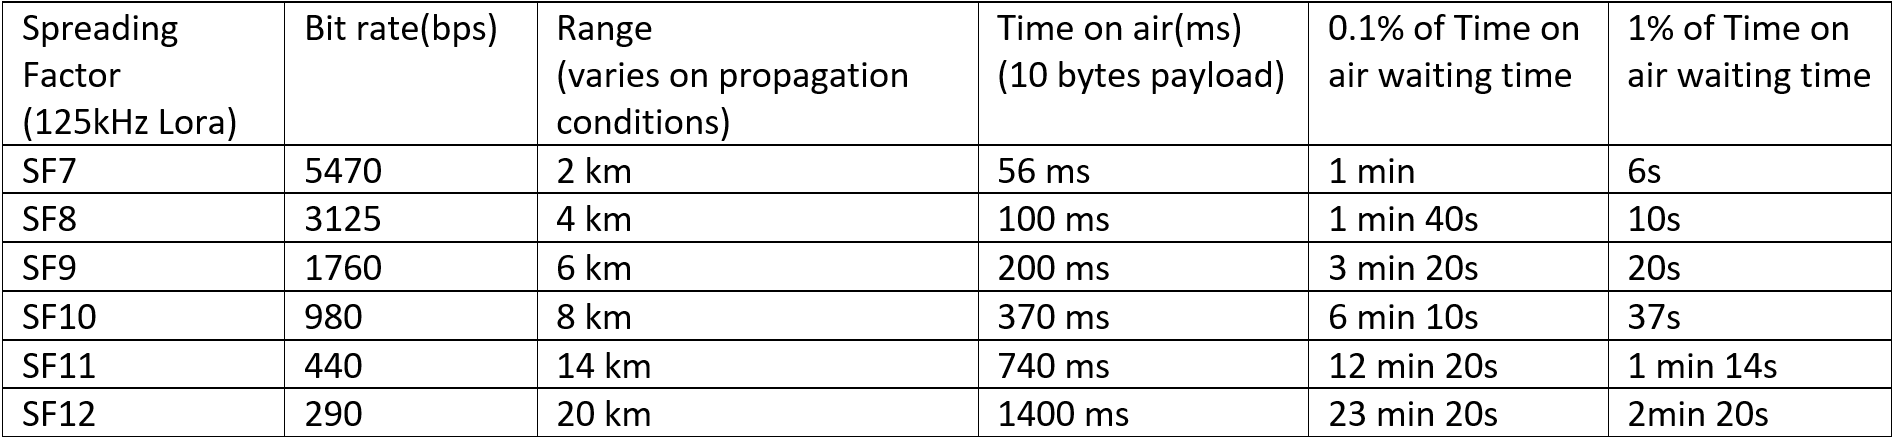
\includegraphics[width=1\textwidth]{spreading_factor_lorawan_2017-07-29}
%     \caption{LoRa spread factor options \cite{24}}
%     \label{fig:loraSF}
% \end{figure}

% \cite{19} \cite{20} \cite{21} \cite{22} \cite{23} \cite{24}.


\subsection{Zigbee}
Zigbee je specifikace navržena pro IoT aplikace, založena na standardu  IEEE 802.15.4, vyvinuta Zigbee alliancí \cite{Zigbee_alliance}, vetšinou používána pro realizaci meshových sítí.
Dostupné transceivery na trhu se pohybují okolo \$8–30 od více různých výrobců, taktéž je i na trhu dostupnýchmnoho Zigbee koncových zařízení.


\subsection{BLE}
Bluetooth Low Energy (BLE) je verze Bluetooth s rádiem navrženým pro minimální spotřebu energie, umožňující topologie point-to-point, broadcast a mesh \cite{BT_alliance}.
Dostupné transceivery na trhu se pohybují okolo \$5–20 od více různých výrobců. Stejně tak je i na trhu mnoho dostupných koncových zařízení, ale mnohdy jsou tato koncová zařízení kompatibilní pouze se zařízení v rámci jednoho výrobce, tudíž může být problém je implementovat do vlastní senzorové sítě. 



% \subsection{Z-Wawe}
% Z-Wave is intended for wireless connectivity for all possible smart home products, controlled by PC, phone, voice, etc. It's based on mesh network topology so every non-battery powered device works as a router to enhance the network range so the more devices are connected in one network, the stronger the network is \cite{27} \cite{28}.
% \subsection{Thread}
% This technology based on IPv6 was developed for home network controlled by smartphone, tablet or PC \cite{29} \cite{30} \cite{31}.


\section{Shrnutí vlastností vybraných technologií}
V tabulce \ref{tab:shrnutiTechnologii} jsou shrnuty vlastnosti zmíněných technologií.   


\begin{table}[]
  \begin{tabular}{|p{1.5cm}||p{2cm}|p{2cm}|p{2cm}|p{2cm}|p{2cm}|}
  \hline
  Technology    & topology options                & frequency bands  & range                                           & price per one transciever & availability of devices on the market \\ \hline \hline
  IQRF           & mesh, star                      & 868 MHz (Europe) & 10-100 m (in building), 100-1000 m (open space) & 15 – 20 \$                & very low                              \\ \hline
  wireless M-bus & star                            & 868M, 433M, 169M & 500 m (868 MHz), 2000 m (169 MHz)               & 25 – 30 \$                & low                                   \\ \hline
  ZigBee         & mesh, star                      & 2.4 GHz          & 100 m (open space)                              & 8 – 30 \$                 & high                                  \\ \hline
  BLE            & Point-to-Point, Broadcast, Mesh & 2.4 GHz          & 100 m (open space)                              & 5 – 20 \$                 & high                                  \\ \hline
  LoRa           & star                            & 868 MHz (Europe) & 15-22 km suburban, 3-8 km urban                 & 5 – 50 \$                 & medium                                \\ \hline
  \end{tabular}
  \caption{Shrnutí vlastností vybraných technologií}
  \label{tab:shrnutiTechnologii}
\end{table}


\section{Vybraná přenosová technologie}
% \section{Wireless Sensor Network Design}
Wireless sensor network design is based on a popular IoT technology LoRa, which is a LPWAN technology using ISM band, 433 MHz, 868 MHz and 915 MHz (depends on the region) and communicates on multiple frequency channels and uses multiple data rates \cite{LoRaWAN Evaluation for IoT Communications}.
The LoRaWAN is an open standard network protocol and system architecture specified by \cite{LoRaWAN specification} and creates a media access control (MAC) layer on the top of the LoRa physical layer, secured by AES-128 encryption.
The LoRaWAN nodes communicate directly with the LoRaWAN gateway \cite{Internet of Things (IoT) using LoRa technology}.




%%%%%%%%%%%%%%%%%%%%%%%%
\part{Practical part}

\chapter{Realizace zařízení}

%%%%%%%%%%%%%%%%%%%%%%%%%%%%%%%%%%%%%%%%%%%%%%%%%%%%%%%%%%%%%%%%%%%%%%%%%%%%%%%%%%%%%%%
\section{Implementace WSN do přístupového systému}
Přístupový systém k rozšíření o WSN pro tento projekt je vytvořen firmou IMA a je komernčně distribuován. Jeho architektura se liší od všeobecné architektury zobrazené v blokovém schematu \ref{fig:Access control system architecture} přidáním zařízení CKP, tvořícího rozhranní mezi kontrolním panelem a čtečkou s dveřním zámkem. Přístupový systém má několik typů CKP zařízení podporujících různé typy čteček, dveřních zámků, závor, vrat apodobně, ale všechna tato CKP zařízení podporují CKP protokol v síti RS485 pro komunikaci s kontrolním panelem.

Rozšíření tohoto Přístupového systému o WSN je vytvořeno připojením WSN gatewaye ke kontrolnímu panelu přes RS485 síť stejně jako CKP zařízení. Názorná blokové schéma přístupového systému firmy IMA s implementací WSN gatewaye je zobrazeno v obrázku \ref{fig:ACS architecture IMA with geteway}.
V budovách, kde již je tento přístupový systém nainstalován je obvykle více kontrolních panelů, vždy jeden kontrolní panel pro několik dveří s CKP zařízeními propojenými sítí RS485. 
K jednomu přístupovému systému je možné přípojit několik WSN gatewayí k libovolným kontrolním panelům v budově pro dosažení požadovaného pokrytí WSN.

\begin{figure}[!h]
\centering
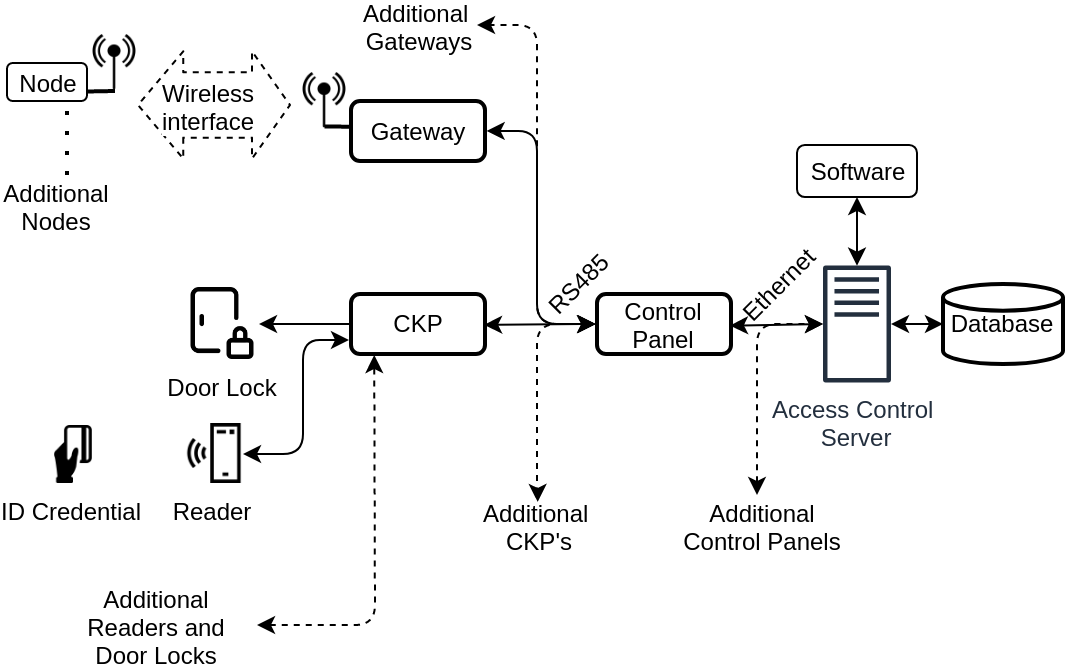
\includegraphics[width=1\textwidth]{ACS_IoT_extension_21}
\caption{IMA access control system architecture with WSN extension}
\label{fig:ACS architecture IMA with geteway}
\end{figure}


WSN gateway tedy musí podporovat CKP protokol v sítí RS485 navržen firmou IMA. Jedná se o kolizní protokol, kde všechna zařízení se řídí pravidlem "listen before talk", kolize jsou detekovány 
mechanismem kontroly integrity použitý v každé zprávě. V případě že zařízení přijme poškozený příkaz, vyžádá jeho opakování.

Přístupový systém firmy IMA funguje tak, že CKP zařízení získává seznam všech platných karet (ID Credentials) ze serveru řízení přístupu a na základě tohoto seznamu pak CKP zařízení provádí odpovídající akci po přiložení karty ke čtečce. 
Je-li ke čtečce přiložena karta, jejíž číslo není obsaženo v seznamu platných karet, CKP zařízení pouze signalizuje událost uživateli (např. červené bliknutí nebo pípnutí), ale zprávu o této události neodesílá na server řízení přístupu. Je-li ke čtečce přiložena karta, jejíž číslo je obsaženo v seznamu platných karet, CKP zařízení signalizuje událost uživateli (např. zelené bliknutí nebo pípnutí) a zprávu o této události odesílá na server řízení přistupu příkazem tzv. "průchod".
Navržená gateway bere seznam platných karet jako seznam platných koncových zařízení senzorové sítě. Gateway pak zpracovává packety pouze od zařízení z tohoto seznamu a ostatní ignoruje, tudíž v síti RS485 jsou přenášena pouze relevantní data.
Data z koncových zařízení jsou odesílána na server řízení přístupu příkazem "průchod", který má fixní velikost a po přidání adresy koncového zařízení o velikosti 4 B zde už zbývá poze 6 B pro data z koncového zařízení, což je velké omezení.
%Since the CKP protocol allows to transmit fixed-size command with only 10 bytes of space, the first 4 bytes are LoRaWAN device address of the node from which the packet was received and the 6 remaining bytes are used for the node data.
LoRaWAN protokol používá packet, jehož samotná hlavička je o minimální velikosti 13 B. 
Různá LoRaWAN koncová zařízení používají různé velikosti payloadu, takže není možné odesílat celý payload koncového zařízení přes síť RS485.
Tento problěm je řešen ta, že LoRaWAN packety z koncových zařízení jsou dešifrovány přímo v gatewayi a konečné hodnoty senzorů jsou vypočítány z payloadu zařízení na základě dokumentace poskytnuté výrobcem \cite{RHF1S001 pdf}. Vybrané hodnoty jsou odeslány na server řízení přístupu skrze kontrolní panel. 
% In summary, when the Gateway receives an encrypted LoRaWAN packet, it looks for whether the Node device address is in the list of known device addresses.
% If this is the case, the packet is encoded in the communication protocol of the Gateway and sent to the Control Panel. If there is not enough space in communication protocol of the Gateway, the packet is decrypted and relevant data, i.e., sensor values, are selected.

% When the user presents his card to the Reader and the card ID matches one of the valid cards, the CKP device sends the data to the Access Control Server.
% The same procedure applies to the Gateway.
% When the Gateway receives data from a Node and the Node address matches one of the valid device address list, the Gateway sends the data to the Access Control Server.

%%%%%%%%%%%%%%%%%%%%%%%%%%%%%%%%%%%%%%%%%%%%%%%%%%%%%%%%%%%%%%%%%%%%%%%%%%
\section{Návrh WSN gatewaye}
Jak již bylo zmíňeno v předchozí sekci, gateway dešifruje packety z koncových zařízení a na základě typu koncového zařízení vypočítává z payloadu hodnoty senzorů z nichž vybrané odesílá na server řízení přístupu přes kontolní panel a to z důvodu datového omezení protokolu v síti RS485, do které je gateway připojena.
Pro každý podporovaný typ koncového zařízení musí být implementováno zpracování payloadu ve FW gatewaye. Pozdější přidání typů koncových zařízení tedy vyžaduje update FW gatewaye.
Gateway tedy má uloženou informaci o typu koncového zařízení společně s jeho LoRaWAN device address.

LoRaWAN protokol je zabezpečen šifrováním AES-128 na dva způsoby, a to zabezpečení aplikační pro nečitelnst přenášených dat a síťové pro zabránění pro zabránění útočníkům opakovat již přenesené packety nebo odesílat falešné packety. Jsou zde tedy dva AES-128 šifrovací klíče, applikační klič AppSKey (Application Session Key) a síťový klíč NwKSKey (Network Session Key).

Jelikož adresy koncových zařízení jsou předávány gatewayi stejně jako platné karty čtečce z aplikace na serveru řízení přistupu, není zde možnost předávávat dva 16 B dlouhé šifrovací klíče pro každé koncové zařízení společně s adresou zařízení. Geteway tedy má tyto dva klíče pro všechna zařízení stejné, uložené v non-volatile paměti, konfigurovatelné pouze přímo na gatewayi.
% LoRaWAN device address a typ každého zařízení v síti je uložena v EEPROM (non-volatile) paměti gatewaye a jsou nastavována na z access control serveru.
% Pro tento projekt byla vyvinuta knihovna pro dekódování payloadu na základě dokumentů \cite{lwSpec} \cite{lwSecur}.
V tomto návrhu neni implementován opačný směr komunikace, tedy ze serveru řízení přístupu na koncové zařízení, ale je také možné implementovat pro ovládání aktulátorů, jako je relé, motor, apod.

%%%%%%%%%%%%%%%%%%%%%%%%%%%%%%%%%%%%%%%%%%%%%%%%%%%%%%%%%%%%%%%%%%%%%%%%%%
\subsubsection{Stavba gatewaye}
% To test the proposed system design, the Gateway is built from one NUCLEO-L073RZ development board \cite{nucleoST}, RFM95w LoRa Shield \cite{RFM95w} and RS485 transceiver \cite{rs485tr}, Fig. \ref{fig:gatewayBlockDiagram}.


% \begin{figure*}[!ht]
%     \centering
%     \includegraphics[width=0.9\textwidth]{5patro}
%     \caption{Location of sensor nodes and CKP devices on the university floor}
%     \label{fig:CorridorFloorPlan}
% \end{figure*}


% \begin{figure}[!h]
%     \centering
%     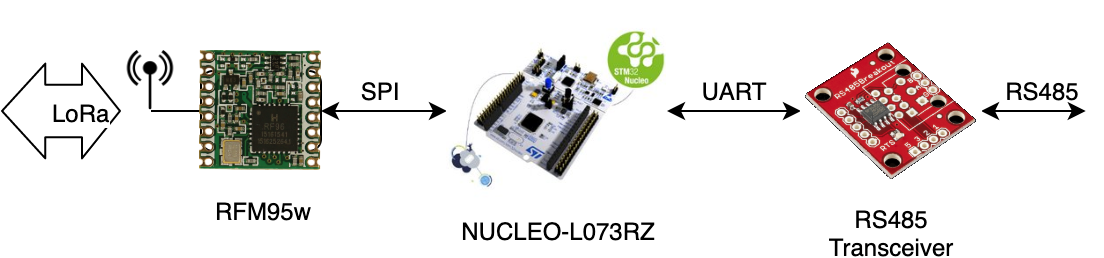
\includegraphics[width=0.48\textwidth]{LoRaWAN_gw_RS485_blockDiagram_2}
%     \caption{Gateway block diagram, RFM95w \cite{RFM95w}, RS485 transceiver \cite{rs485tr}, NUCLEO-L073RZ \cite{nucleoST}}
%     \label{fig:gatewayBlockDiagram}
% \end{figure}

% The NUCLEO-L073RZ development board with STM32L073RZ microcontroller is suitable for the development purposes because of its parameters, Tab. \ref{tab:mcuFeatures}, price and available documentation.
%It is  was used for the prototype, because it has all required parameters, it is cheap, powerful enough and easily prototypable.
% The price of the devlopment board is \$13 USD\cite{nucleoST}.
% LoRa transceiver board RFM95w with SX1276 chip integrated into Dragino LoRa Shield has the same pinout as the NUCLEO-L073RZ development board. RS485 transceiver as an RS485/UART interface enables communication with Control Panel.

%RS485 transceiver SparkFun Breakout is used for the communication with the Control Panel. It converts interfaces UART to RS485, Fig. \ref{fig:gatewayBlockDiagram}.


% \begin{table}[h]
% \centering
% \footnotesize
% \caption{The STM32L073RZ features \cite{nucleoST}}
% \begin{tabular}{|l|p{3.5cm}|}
% \hline
% Microcontroller architecture & ARM Cortex-M0+ 32-bit RISC \\ \hline
% Internal flash memory & 192 KB \\ \hline
% Internal SRAM memory & 20 kB \\ \hline
% Internal EEPROM memory & 6 kB \\ \hline
% CPU frequency & up to 32 MHz \\ \hline
% Interfaces & 2X SPI, 3x I2C, 4x UART, LIN \\ \hline
% \end{tabular}
% \label{tab:mcuFeatures}
% \end{table}

% \section{Výběr komponent}
% \subsection{Microcontroller}
% Pro toto zařízení je zvolen mikrocontroller STM32L073RZ se zaměřením na nízkou spotřebu, jelikož je levný, má dostačující vlastnosti a je dostupný ve formě vývojového kitu NUCLEO-L073RZ který byl použit pro  vývoj zařízení. Mezi hlavní vlastnosti patří \cite{nucleoST}:
% \begin{itemize}    
%     \item {Architektura ARM Cortex-M0+ 32-bit RISC}
%     \item{Interní Flash paměť 192 KB}
%     \item{Interní SRAM paměť 20 KB}
%     \item{Interní EEPROM paměť 6 KB}
%     \item {Až 32 MHz CPU}
%     \item {2X SPI, 3x I2C, 4x USART, LIN, ADC}
% \end{itemize}

% Pořizovací cena kitu přímo na stránce výrobce www.st.com je \$13 \cite{nucleoST} \cite{nucleoMbed}.
% \begin{figure}[!h]
%     \centering
%     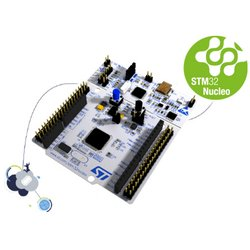
\includegraphics[width=0.4\textwidth]{Nucleo64}
%     \caption{Vývojový kit NUCLEO-L073RZ \cite{nucleoST}}
%     \label{fig:02}
% \end{figure}

% \subsection{LoRa transceiver}
% Lora transceiver čip doposud vyrábí pouze Semtech, pro použití v Evropském pásmu je určen typ SX1276.
% V tomto návrhu je použita deska RFM95w od firmy HopeRF s integrovaným čipem SX1276 \cite{RFM95w}.
% Pro vývoj zařízení byl využit tento transciever v tzv. Dragino LoRa Shield \cite{draginoWiki}, který má stejně jako použitý vývojový kit, pinout kompatibilní s Arduino UNO. Pořizovací cena samotného transceiveru RFM95w je okolo \$7, cena Dragino Shieldu se pohybuje okolo \$22 na ebay.

% \begin{figure}[!h]
%     \centering
%     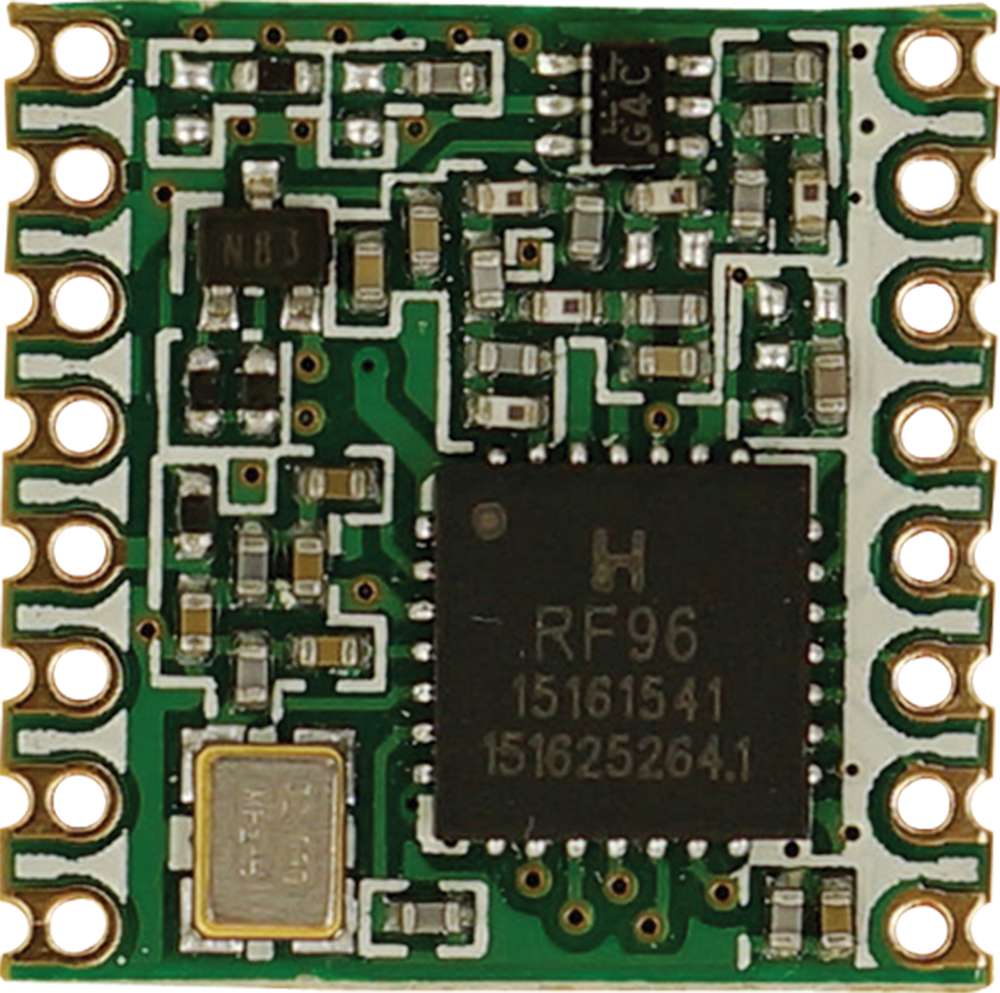
\includegraphics[width=0.2\textwidth]{RFM95w}
%     \caption{LoRa transceiver RFM95w \cite{RFM95w}}
%     \label{fig:02}
% \end{figure}

% \subsection{RS485 transceiver}
% SparkFun Transceiver Breakout - RS485 převádí rozhranní UART na RS485, pří vstupním napětí 3.3 V. A je dostupný za cenu okolo \$10 \cite{rs485tr}.

% \begin{figure}[!h]
%     \centering
%     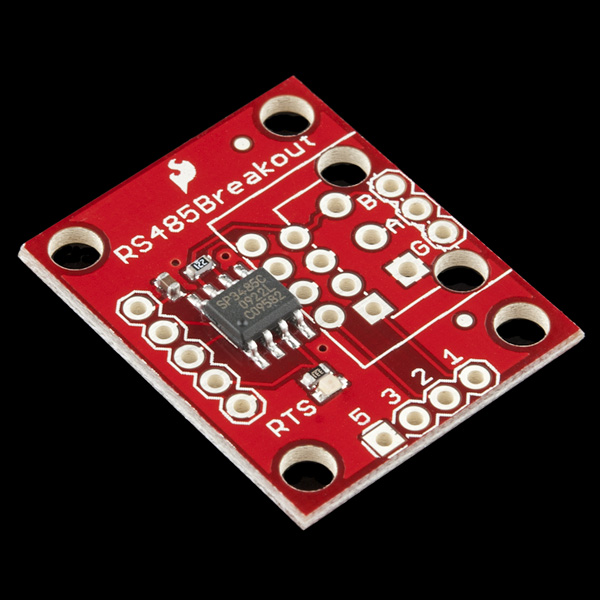
\includegraphics[width=0.4\textwidth]{rs485transceiver}
%     \caption{RS485 transceiver \cite{rs485tr}}
%     \label{fig:rs485transceiver}
% \end{figure}



%%%%%%%%%%%%%%%%%%%%%%%%%%%%%%%%%%%%%%%%%%%%%%%%%%%%%%%%%%%%%%%%%%%%%%%%%%
% \section{Implementace komunkičního protokolu v síti IMA\_RS485 pro komunikaci s control panelem}
% V tomto projektu je komunikace protokolu IMA\_RS485 naprogramována v souborech rs485\_protocol.h a rs485\_protocol.c. 
% Jedná se o kolizní protokol v síti, kde je připojen jedno zařízení typu master, a jeden nebo více zařízení v typu slave.

% \begin{table}[!h]
%     \centering
%     \begin{tabular}{ |c|c| }
%      \hline

%      Baud rate              & 9600           \\ \hline
%      Data bits              & 8                 \\ \hline
%      Parity                 & none              \\ \hline
%      Stop bits              & 1                 \\ \hline

%     \end{tabular}
%     \caption{Fyzické vlastnosti IMA\_RS485 sítě}
%     \label{table:3}
% \end{table}

% \newpage
% \subsection{Syntaxe příkazů}
% Komunikace v síti probíhá formou příkazů, které mají specifikovanou syntaxi v tabulce \ref{table:syntaxePrikazu}.

% \begin{table}[!h]
%     \centering
% \begin{tabular}{ |c|| p{1.5cm} | p{1.5cm} | p{1cm} | p{1cm} | p{1cm} | p{1cm} | }
%  \hline
%  popis      & adresa příjemce & adresa odesílatele & typ příkazu & délka dat & data & crc\\ \hline
%  počet bytů & 1               & 1   & 1     & 2     & délka dat     & 1 \\ 
%  \hline
% \end{tabular}
%     \caption{Syntaxe příkazu pro komunikaci v síti IMA\_RS485}
%     \label{table:syntaxePrikazu}
% \end{table}

% Typy příkazu jsou zadefinované konstanty s předponou CKP\_CMD\_ v souboru ./Inc/rs485\_protocol.h.
% Příkazy odeslané zařízením typu master obsahují navíc synchronizační byte na začátku 0xAA.
% CRC je pro kontrolu XOR přes všechny předchozí byty v celém příkazu kromě synchronizačního bytu.

% \subsection{Adresace zařízení v síti}
% Každé zařízení na této sběrnici má svoji adresu, která mu je nastavena externě. Zařízení typu master má adresu  0xFF, adresa pro všechny (broadcast) je 0x00 a zařízení v této sítí můžou mít adresu libovolnou (krom těchto dvou) nesmí zde však být připojena 2 zařízení s nastavenou stejnou adresou.

% \subsection{Statusy}
% Zařízení typu slave má dva možné statusy v síti IMA\_RS485, offline a online. Zařízení typu slave má povoleno odesílat příkaz "průchod" pouze má-li status online.  
% Zařízení typu slave odesílá příkaz obsahující informaci o jeho statusu periodicky s typem příkazu 0x10 a jedním bytem dat označujícím status. 
% Pro status online je tento byte 0x00 a pro status offline 0xEE. 
% Tento příkaz je odesílán s intervalem 10 s, pokud zařízení má status offline a s intervalem 30 s, pokud má zařízení status online.
% Status zařízení mění pouze zařízení typu master odesláním příkazu s typem 0x41 pro přepnutí na status online a 0x42 pro přepnutí na status offline.
% Zařízení typu slave svůj status přepne samo pouze v případě, že má status online a zařízení typu master přestane odpovídat na příkaz průchod, jak je popsáno v sekci \ref{sec:Odesílání dat z koncových zařízení}.
% Je-li zařízení spuštěno, je ve stavu offline a jelikož nemá povoleno odesílat příkaz "průchod", přijatá data z koncových zařízení jsou zahazována. 
% Zařízení typu slave pouze odpovídá na příkazy od zařízení typu master a čeká na příkaz od zařízení typu master k přepnutí na status online.


% \subsection{Přidávání LoRaWAN zařízení do systému}
% Pokud zařízení typu master přijme příkaz od zařízení typu slave oznamující že je ve stavu offline, nejprve tomuto zařízení pošle seznam LoRaWAN adres všech známých koncových zařízení a následně toto zařízení přepne do stavu online.
% Přijímání seznamu adres je realizováno sekvencí příkazů typu 0x8F. 

% Níže v tabulce \ref{table:2} je příklad sekvence příkazů odesílaných mezi zařízením typu masterem a zařízením typu slavem během předávání seznamu LoRaWAN device address koncových zařízení, kde zařízení typu slave má adresu 0x10 a zařízení typu master standardně 0xFF. Jak již bylo řečeno, příkazy od zařízení typu master lze jednoduše odlišit tím, že vždy začínají bytem 0xAA.


% \begin{table}[!h]
%     \begin{tabular}{ |l|p{10cm}| }
%     \hline
%     příkaz      &  data    \\ \hline \hline
%     master: start      &  AA 10 FF 8F 02 00 00 00 62    \\ \hline
%     slave: ACK        &  FF 10 06 02 00 8F 00 64    \\ \hline
%     master: data     &  AA 10 FF 8F 21 00 01 B1 C4 12 00 00 00 00 00 B2 C4 12 00 00 00 00 00 B3 C4 12 00 00 00 00 00 B4 C4 12 00 00 00 00 00 44 \\ \hline
%     slave: ACK      &  FF 10 06 02 00 8F 01 65   \\ \hline
%     master: data     &  AA 10 FF 8F 19 00 02 B5 C4 12 00 00 00 00 00 B6 C4 12 00 00 00 00 00 F6 1F 01 26 00 00 00 00 B6 \\ \hline
%     slave: ACK      &   FF 10 06 02 00 8F 02 66   \\ \hline
%     master: konec   &   AA 10 FF 8F 04 00 03 FF 2A 57 E5   \\ \hline
%     slave: ACK      &   FF 10 06 02 00 8F 03 67  \\ \hline
%     \end{tabular}
%     \caption{Příklad sekvence příkazů odesílaných mezi zařízením typu master a zařízením typu slave během předávání seznamu LoRaWAN device address koncových zařízení}
%     \label{table:2}
% \end{table}

% LoraWAN protokol používá 4-bytové adresy koncových zařízení.
% Adresy předávány touto sekvencí jsou dlouhé 8-bytové. První 4 byty je tedy LoRaWAN device address, pátý byte je typ zařízení a zbylé 3 byty jsou nevyužity, jejich použití je možné v případě změn či rozšiřování vlastností systému. 

% První Byte dat je counter paketu začínající od nuly, který označuje číslo odeslaného paketu v sekvenci. Na každý tento paket v sekvenci zařízení typu slave odpovídá ACK příkaz, který se liší od obyčejného ACK příkazu tím, že v datech paketu navíc obsahuje counter pakety v sekvenci.
% První příkaz této sekvence má délku dat 2 byty, které mají hodnotu 0x00 přičemž první je counter.
% Další příkazy hned za counter bytem obsahují několik osmibytových adres, jejichž počet je různý.
% Příkaz ukončující tuto sekvenci příkazů má délku 4 byty, což je tedy counter, 0xFF a 2 byty CRC přes všechny odeslané adresy (nepodstatné, tudíž ho nepoužívám).

% \subsection{Odesílání dat z koncových zařízení} 
% \label{sec:Odesílání dat z koncových zařízení}
% Jak je popsáno v sekci \ref{sec:Implementace IoT do přístupového systému firmy IMA}, tudíž data z koncových zařízení jsou odesílána příkazem "průchod", jehož typ je 0x10 a kapacita na data z koncového zařízení je pouze 6 B. 
% První byte dat označuje typ průchodu, byl zvolen konstantní byte 0xD0. Dále následuje LoRaWAN adresa koncového zařízení od kterého byl paket přijat. Dále následují 4 byty dat ze senzoru, další 2 byty signalizující čas průchodu, což v tomto projektu není použito a tyto dva byty mají vždy hodnotu 0xFF. A nakonec jsou další 2 byty obsahující data ze senzoru.
% Příklad příkazu: FF 1F 10 0D 00 D0 F6 1F 01 29 AD 0A 5A 27 FF FF DE 09 E1.
% Data příkazu jsou níže rozepsána v tabulce \ref{table:prikladprikazpruchod}.

% \begin{table}[!h]
%     \centering
% \begin{tabular}{ | p{1.5cm} | p{3cm} | p{2.5cm} | p{1.3cm} | p{1.3cm} |  }
%  \hline
%  typ průchodu & LoRaWAN device address & data (4B)     & cas   & data (2B) \\ \hline
%  D0           & F6 1F 01 29            &  AD 0A 5A 27  & FF FF & DE 09     \\ 
%  \hline
% \end{tabular}
%     \caption{Příklad dat příkazu "průchod" odeslaného z gatewaye na zarizeni typu master, obsahující data z koncových zařízení}
%     \label{table:prikladprikazpruchod}
% \end{table}

% Zařízení typu master na příkaz "průchod" odpovídá příkazem ACK. Zařízení typu slave na tuto odpověď čeká standardně 3 sekundy, ale tento parametr je nastavitelný. Pokud v tomto timeoutu zařízení typu master neodpoví, zařízení typu slave příkaz "průchod" zopakuje přičemž změní typ příkazu na 0x20. Pokud zařízení typu master ani na třetí opakování neodpoví ACK, zařízení typu slave se přepne do stavu offline a vymaže frontu příkazů "průchod" k odeslání.

% \subsection{Potvrzení}
% Zařízení typu slave odpovídá na každý příkaz od zařízení typu master ACK. Typ příkazu ACK je 0x06 a data příkazu obsahují jeden byte signalizující typ příkazu na který je právě odpovídáno potvrzením.
% Zařízení typu master odpovídá ACK se stejným typem příkazu 0x06, ale s žádnými daty příkazu.

% \subsection{Dotaz na příznaky}
% Zařízení typu master se může zeptat s jak dlouhými adresami zařízení typu slave pracuje s typem příkazu 0x49. Zařízení typu slave na to odpovídá ACK s tím, že v datech příkazu je navíc byte 0x04. Zařízení typu master pak počítá s tím, že zařízení typu slave pracuje se 64-bit adresami (ve skutečnosti ale používá 32-bitové a zbylé 4 byty v příkazu průchod jsou pro data z koncového zařízení).

%%%%%%%%%%%%%%%%%%%%%%%%%%%%%%%%%%%%%%%%%%%%%%%%%%%%%%
\subsection{Komunikace přes sériovou linku}
\label{Komunikace přes sériovou linku}
Gateway má implementovanou komunikaci přes sériovou linku, umožňující konfiguraci a log. 
K přípojení lze použít PC s libovolnou aplikací umožňující obousměrnou komunikaci přes sériovou linku s nastavením parametrů dle tabulky \ref{table:usb_term}.

\begin{table}[!h]
    \centering
    \begin{ctucolortab}
    \begin{tabular}{ |c|c| }
     \hline

     Baud rate              & 115200           \\ \hline
     Data bits              & 8                 \\ \hline
     Parity                 & none              \\ \hline
     Stop bits              & 1                 \\ \hline
     Flow control           & none               \\ \hline

    \end{tabular}
    \end{ctucolortab}
    \caption{Parametry sériové linky PC terminálu pro komunikaci s gatewayí}
    \label{table:usb_term}
\end{table}

Při komunikaci jsou data standardně oddělována bytem CR (carriage return) 0x0D, ale je akceptována i sekvence CR LF (Line Feed), tedy 0x0D 0x0A. 

%%%%%%%%%%%%%%%%%%%%%%%%%%%%%%%%%%%%%%%%%%%%%%%%%%%%%
\section{Log Gatewaye}
Po připojení ke gatewayi přes sériovou linku dle instrukcí v sekci \nameref{Komunikace přes sériovou linku} je možné kontinuálně snímat a log gatewaye obsahující informace o proběhlých událostech.
Níže je příklad výpisu logu pro případ, že gateway přjala LoRaWAN paket z koncového zařízení senzorové sítě, zpracovala ho a výslednou informaci odeslala na kontrolní panel přes RS485 síť.

% ______________________________________________________
% \begin{ctucolortab}
\begin{lstlisting}[style=log]

________________________________________________
Rx -> LoRaWAN, pktCntr: 6
RSSI: -51, SNR: 9, length: 22

Message type: Unconfirmed Data Up
Packet rawData: "40F61F0128C0D62508D970CB071595D115BAC68F6663"
Device Address: "F61F0128"
FCnt: 9686
message (encrypted): "D970CB071595D115BA"
MHDR: 40; FCtrl: C0; FPort: 08; MIC: "C68F6663"
adaptive data rate: true; ack: false
message HEX (decrypted): "013566779600FFFFAF"

Sensor type: RHF1S001
temperature: 23.30 C, humidity: 52 %
period: 300 s, RSSI: -51 dBm, SNR: 9 dB, battery voltage: 3.2 V
Tx -> RS-485: "FF1F100D00D0F61F01281A0934CDFFFF09202E"
________________________________________________
Rx -> RS-485: "AA1FFF060000E6"
ACK
\end{lstlisting}
% \end{ctucolortab}


Nejprve jsou vypsána data týkající se LoRaWAN protokolu, zašifrovaný i dešifrovaný payload, typ zařízení a konečné informace dekódované z payloadu.
Řádek začínajci předponou "Tx -> RS-485:" obsahuje data odeslané k zařízení typu master přes RS485 síť a následující řádek začínající předponou "Rx -> RS-485:" obsahuje odpověď od zařízení typu master.


%%%%%%%%%%%%%%%%%%%%%%%%%%
% \subsection{Konfigurace systému}
% \label{sec:konfigurace}
% Konfigurace gatewaye se provádí opět přes USB port. Je do ní vstoupeno odesláním příkazu
% "config", následuje vypsání současného stavu konfigurace a dále je vypsáno konfigurační menu, kde uživatel vybere jednotlivý bod menu zadáním jeho čísla na začátku řádku.
% Níže je zobrazen příklad výpisu po vstupu do konfigurace.

% \begin{lstlisting}
%     _________________Entering configuration setup________________

%     System configuration:

%     *** LoRa channel: 
%     channel: 0 (868.1 Mhz)
%     SF7

%     *** RS485 channel: 
%     my address: 10
%     master address: FF
%     timeout: 3 s

%     *** LoRaWAN keys: 
%     NwSKey:  FD 90 0D 8C 70 9F 19 24 18 EC FD D4 28 0C AC 47
%     AppSKey:  68 9F D0 AC 7A 0F 95 58 B1 19 A0 16 17 F4 16 33

    
%     Config menu:
%     1 -> Config LoRa channel
%     2 -> Config RS485 channel
%     3 -> Config LoRaWAN protocol
%     4 -> Print all LoRaWAN devices
%     5 -> Erase all LoRaWAN devices
%     6 -> Restore to default configuration
%     7 -> Exit without save
%     8 -> Save and exit
% \end{lstlisting}


% Z konfigurace je možné vystoupit kdykoliv bez uložení změn příkazem "quit". 
% Při vstoupení do konfigurace je pozastavena činnost gatewaye, komunikace s koncovými zařízeními LoRaWAN síťě a komunikace se zařízením typu master v síti RS485 nejsou aktivní.
% Jsou zde tedy 3 stavy konfigurace, přičemž je možné vždy jednotlivá nastavení přeskakovat odesláním "prázdného příkazu" 0x0D (v terminálu obvykle stačí stisknout Enter). Systém při konfiguraci vždy vypíše jaká data mají být zadána v jakém tvaru a zároveň současnou hodnotu měněného parametru. Zadaná data uživatelem jsou vždy zkontrolována zda splňují požadovaný tvar. Pokud ne, uživatel je o tom informován a vyzván k dalšímu pokusu.
% Po provedení konfigurace následuje vždy návrat zpět do hlavního menu. Pro uložení nové konfigurace je potřeba v menu vybrat "Save and exit", gateway pak následně vypíše které parametry byly změněny a provede restart.

% \subsubsection{Config LoRa channel}
% Konfigurace LoRa RF kanálu zahrnuje nastavení SF a frekvenční pásmo. Níže je příklad konfigurace.

% \begin{lstlisting}
% LoRa channel configuration:
% Enter SF number (7-12)
% (current: 7)
% 8
% SF8 set.

% Enter LoRa channel number (0-7)
% ch0 is 868.1 Mhz
% ch1 is 868.3 Mhz
% ch2 is 868.5 Mhz
% ch3 is 867.1 Mhz
% ch4 is 867.3 Mhz
% ch5 is 867.5 Mhz
% ch6 is 867.7 Mhz
% ch7 is 869.0 Mhz
% (current: 0)
% 1
% channel 1 set.
% \end{lstlisting}

% \subsubsection{Config RS485 channel}
% Konfigurace RS485 kanálu pro komunikaci se zařízením typu master zahrnuje nastavení adresy tohoto zařízení, adresa zařízení typu master a timeout, což je doba čekání na potvrzení od zařízení typu master po odeslání příkazu "průchod". Níže je příklad konfigurace.

% \begin{lstlisting}
% RS485 channel configuration:
% Enter address of this device, FF and 00 are reserved.
% (current: 10)
% 11
% Address of this device is set to: 11

% Enter master address: 
% (current: FF)
% FE
% Master address is set to: FE

% Enter timeout (seconds)
% (current: 3)
% 5
% timeout set to: 5 s
% \end{lstlisting}


% \subsubsection{Config LoRaWAN protocol}
% Konfigurace LoRaWAN protokolu zahrnuje nastavení šifrovacích klíčů NwkSKey a AppSKey. Níže je příklad konfigurace.

% \begin{lstlisting}
% LoRaWAN protocol configuration:
% Enter NwkSKey (16 bytes in HEX)
% (current:  FD 90 0D 8C 70 9F 19 24 18 EC FD D4 28 0C AC 47)
% 11111111222222223333333344444444
% NwSKey set to: 11 11 11 11 22 22 22 22 33 33 33 33 44 44 44 44

% Enter AppSKey (16 bytes in HEX)
% (current:  68 9F D0 AC 7A 0F 95 58 B1 19 A0 16 17 F4 16 33)
% 11111111222222223333333344444444
% AppSKey set to: 11 11 11 11 22 22 22 22 33 33 33 33 44 44 44 44
% \end{lstlisting}


% \subsubsection{Print all LoRaWAN devices}
% Vypíše všechna LoRaWAN zařízení uložená v paměti. Níže je příklad.


% \begin{lstlisting}
% number.......................0:
% Device Address:  B1 C4 12 00
% Device Type: RH1S001
% number.......................1:
% Device Address:  B2 C4 12 00
% Device Type: RH1S001
% number.......................2:
% Device Address:  B3 C4 12 00
% Device Type: RH1S001
% number.......................3:
% Device Address:  B4 C4 12 00
% Device Type: IMA_tempPress
% number.......................4:
% Device Address:  B5 C4 12 00
% Device Type: IMA_tempPress
% \end{lstlisting}



% \subsubsection{Restore default configuration}
% Po zvolení této možnosti je načtena defaultní konfigurace systému, která obsahuje hodnoty viz tabulka \ref{table:5}. Tyto defaultní hodnoty jsou nastaveny v programu a slouží především pro testovací účely.

% \begin{table}[!h]
%     \centering
%     \begin{tabular}{ |l|l| }
%      \hline

%      popis              & hodnota         \\ \hline \hline
%      RS485 myAddr       & 0x10            \\ \hline
%      RS485 MasterAddr   & 0xFF            \\ \hline
%      RS485 timeout      & 3               \\ \hline
%      LoRa SF            & SF7             \\ \hline
%      LoRa channel       & 0 (868.1 Mhz)   \\ \hline
%      NwSKey             & FD 90 0D 8C 70 9F 19 24 18 EC FD D4 28 0C AC 47  \\ \hline
%      AppSKey            & 68 9F D0 AC 7A 0F 95 58 B1 19 A0 16 17 F4 16 33  \\ \hline

%     \end{tabular}
%     \caption{Defaultní konfigurace systému}
%     \label{table:5}
% \end{table}


% \newpage
%%%%%%%%%%%%%%%%%%%%%%%%%%%%%%%%%%%%%%%%%%%%%%%%%%%%%%
% \section{Koncová zařízení}
% Jelikož používaný protokol ke komunikaci se zařízením typu master je omezen na pouhých 6 B na jeden paket, payload koncových zařízení je dekódován v gatewayi a v paketu odeslaném na zařízení typu master jsou pouze vybraná nejdůležitější data, která se vejdou do této velikosti.
% Prote společně s LoRaWAN device address koncového zařízení je v gatewayi uložen i typ zařízení zadefinován jedním bytem a na základě typu zařízení gateway rozpozná jak dekódovat payload.

% Momentálně jsou podporovány dva typy koncových zařízení, dle potřeby je možné rozšířit FW gatewaye o další typy koncových zařízení.

% \begin{table}[!h]
%     \centering
%     \begin{tabular}{ |l|l| }
%      \hline

%      Typ zařízení       & Hodnota         \\ \hline \hline
%      RHF1S001           & 0x00            \\ \hline
%      IMA\_tempPress     & 0x01            \\ \hline

%     \end{tabular}
%     \caption{Typy koncových zařízení}
%     \label{table:TypyKoncZarizeni}
% \end{table}

% \subsection{Zpracování dat jednotlivých typů koncových zařízení}
% Níže je popsáno pro jednotlivá podporovaná koncová zařízení jak jsou data uložena v datové struktuře, jak jsou data z této struktury zpracována a zobrazena a nakonec jak vybraná data jsou zapsána do výsledného bufferu o délce 6 B, který je odeslán na zařízení typu master příkazem "průchod".

\subsubsection{RHF1S001}
Senzor od firmy RisingHF měří teplotu a vlhkost.


\begin{lstlisting}[style=CStyle]
    /* RHF1S001 data structure */   
    typedef struct {
        int16_t temperature;
        uint8_t humidity;
        uint16_t period;
        int8_t rssi;
        int8_t snr;
        uint8_t battery;
    } RHF1S001_data_t;

    /* Print the data from the structure */
    printf("temperature: %d.%d C, ", RHF1S001_data.temperature / 100, RHF1S001_data.temperature % 100);
    printf("humidity: %d %%\n", RHF1S001_data.humidity);
    printf("period: %d s, ", (int)RHF1S001_data.period);
    printf("RSSI: %d dBm, ", RHF1S001_data.rssi);
    printf("SNR: %d dB, ", RHF1S001_data.snr);
    printf("battery voltage: %d.%d V\r\n", RHF1S001_data.battery/10, RHF1S001_data.battery % 10);

    /* Put the data into 6B long buffer, that is transmitted to the master */
    buffer[0] = RHF1S001_data.temperature & 0xFF;
    buffer[1] = RHF1S001_data.temperature >> 8;
    buffer[2] = RHF1S001_data.humidity;
    buffer[3] = RHF1S001_data.rssi;
    buffer[4] = RHF1S001_data.snr;
    buffer[5] = RHF1S001_data.battery;
\end{lstlisting}


% \subsubsection{IMA\_tempPress}
% Senzor vytvořený ve firmě IMA, měřící teplotu a tlak.

% \begin{lstlisting}[style=CStyle]
%     /* IMA_tempPress data structure */   
%     typedef struct {
%         int16_t temperature;
%         uint16_t pressure;
%         int8_t rssi;
%         int8_t snr;
%     } IMA_tempPress_data_t;

%     /* print the data from the structure */
%     printf("temperature: %d.%d C, ", IMA_tempPress_data.temperature / 100, IMA_tempPress_data.temperature % 100);
%     printf("pressure: %d.%d Pa\r\n", IMA_tempPress_data.pressure/10, IMA_tempPress_data.pressure % 10);
%     printf("RSSI: %d dBm, SNR: %d dB\r\n", IMA_tempPress_data.rssi, IMA_tempPress_data.snr);

%     /* Put the data into 6B long buffer, that is transmitted to the K4 server */
%     buffer[0] = IMA_tempPress_data.temperature & 0xFF;
%     buffer[1] = IMA_tempPress_data.temperature >> 8;
%     buffer[2] = IMA_tempPress_data.pressure & 0xFF;
%     buffer[3] = IMA_tempPress_data.pressure >> 8;
%     buffer[4] = IMA_tempPress_data.rssi;
%     buffer[5] = IMA_tempPress_data.snr;
% \end{lstlisting}


\subsection{Přidávání koncových zařízení ze serveru řízení přístupu K4}
% Koncocová zařízení sítě se nastavují ze serveru K4 v podobě seznamu offline karet s délkou UID 8 B.
% LoRaWAN device address je dlouhá 4 B, jeden byte je navíc použit pro typ koncového zařízení, zbylé 3 byty jsou nuly.
% Jelikož typ zařízení je uložen v gatewayi i na K4 serveru. Při odesílání příkazu průchod se tedy už typ zařízení neposílá z důvodu datového omezení tohoto příkazu.
% Na serveru K4 se UID nastavuje jako dekadické číslo.
% Níže je příklad vytvoření výsledného čísla obsahující DevAddr a typ zařízení, které se zadává do K4 serveru.

% \subsubsection{Příklad}
% Pro případ, kde typ zařízení je 01 a DevAddr AABBCCDD (little endian) výsledné číslo v hexadecimální podobě je 01DDCCBBAA. Následně se překládá do decimalni podoby, výsledné číslo k zadání do K4 serveru je tedy 8016149418.


%%%%%%%%%%%%%%%%%%%%%%%%%%%%%%%%%%%%%%%%%%%%%%%%%%%%%%
% \section{Využití non-volatile paměťi gatewaye}
% Konfigurace a adresy s typy všech koncových zařízení v LoRaWAN síti jsou uloženy v non-volatile paměti EEPROM gatewaye o kapacitě 6144 B. 
% Paměť je tedy rozdělená tak, že od adresy 0 až po 6080 je prostor pro ukládání LoRaWAN zařízení a od 6080 až po 6144 je prostor pro ukládání konfigurace gatewaye.

% Každé LoRaWan zařízení v síti má v paměti uložené LoRaWAN device address (4 byty), typ zařízení (1 byte) a další 3 byty jsou rezervovány. 
% Jedno koncové zařízení v paměti tedy zabírá  8 B, takže gateway má kapacitu paměti pro až 760 koncových zařízení.


%%%%%%%%%%%%%%%%%%%%%%%%%%%%%%%%%%%%%%%%%%%%%%%%%%%%%%
% \section{Zapojení}
% LoRa shield \cite{draginoWiki} je nasazen přímo na vývojový kit Nukleo. Kit neobsahuje ISCP konektor, který je součástí pinoutu Arduino UNO a LoRa shield má SPI piny MISO a MOSI přivedeny právě na tento konektor. Musí být tedy propojeny externě viz obrázek \ref{fig:03}. Jumpery na Dragino LoRa shieldu musí také být stejně jako v obrázku.

% \begin{figure}[!h]
%     \centering
%     \includegraphics[width=1\textwidth]{foto01}
%     \caption{foto zapojení}
%     \label{fig:03}
% \end{figure}

% Pro komunikaci s LoRa transceiverem je tedy použito SPI1, pro komunikaci přes USB je použito USART2 a pro komunikaci přes RS485 je použito UART1.

% \begin{table}[h]
%     \centering
%     \begin{tabular}{ |c|c|c| }
%      \hline

%      Periférie          & Název pinu & Pin procesoru           \\ \hline \hline

%                         & RX  &   PC1            \\
%     RS485 transceiver   & TX  &   PC0       \\
%                         & RTS  &  PB1      \\     \hline

%                         & CS    &  PB6             \\
%                         & CLK   &  PA5        \\
%    LoRa transceiver     & MISO  &  PA6     \\
%                         & MOSI  &  PA7        \\
%                         & RST   & PC7          \\
%                         & DIO0  & PA10         \\
%                         \hline

%     \end{tabular}
%     \caption{Pinout připojení externích periférií k procesoru}
%     \label{table:3}
% \end{table}

%%%%%%%%%%%%%%%%%%%%%%%%%%%%%%%%%%%%%%%%%%%%%%%%
% \section{Naprogramování}
% K naprogramování MCU byla použita HAL knihovna a inicializační nástroj STM32CubeMX poskytnuté výrobcem, tedy ST Microelectronics.
% Zdrojové soubory programu byly vyvíjeny v textovém editoru VS-Code, ke kompilaci zdrojových souborů byl použit kompilátor arm-none-eabi-gcc a jako pomocný nástroj makefile skript. 

% \subsection{Zdrojové soubory projektu}
% Pro šifrování LoRaWAN paketu byla použita knihovna AES-128, dostupná na githubu \cite{AESlib} a knihovna OpenPANA také dostupná z githubu \cite{CMAClib}.
% Níže je seznam zdrojových souborů.

% \begin{figure}[!h]
%     \dirtree{%
%         .1 Drivers \DTcomment{STM32 Drivers}.
%         .1 Inc\DTcomment{Headers}.
%             .2 aes.h\DTcomment{AES-128 library for LoRaWAN paket encryption}.
%             .2 cmac.h\DTcomment{library for CMAC calculation in LoRaWAN protocol}.
%             .2 LinkedList\_ByteArray.h \DTcomment{Byte array linked list library for stacks}.
%             .2 LoRaWAN\_paket.h\DTcomment{LoRaWAN library for paket data decoding}.
%             .2 stm32l0xx\_hal\_conf.h\DTcomment{HAL initialization of peripherals}.
%             .2 ByteArray.h\DTcomment{Library for Byte array operations}.
%             .2 LoRa.h\DTcomment{Library for interfacing LoRa transceiver}.
%             .2 main.h\DTcomment{Main file}.
%             .2 stm32l0xx\_it.h\DTcomment{HAL initialization of peripherals}.
%             .2 eeprom.h\DTcomment{Library for eeprom operations}.
%             .2 LoRa\_sensors.h\DTcomment{Library for decoding data from payload}.
%             .2 rs485\_protocol.h\DTcomment{Library for RS485 IMA protocol}.
%             .2 usb.h \DTcomment{Library for USB communication and system configuration}.
%         .1 Src\DTcomment{Sources}.
%             .2 aes.c \DTcomment{source file to the aes.h}.
%             .2 aes.c \DTcomment{source file to the cmac.h}.
%             .2 LinkedList\_ByteArray.c \DTcomment{source file to the LinkedList\_ByteArray.h}.
%             .2 LoRaWAN\_paket.c  \DTcomment{source file to the LoRaWAN\_paket.h}.
%             .2 stm32l0xx\_hal\_msp.c \DTcomment{HAL source file}.
%             .2 ByteArray.c  \DTcomment{source file to the ByteArray.h}.
%             .2 LoRa.c \DTcomment{source file to the LoRa.h}.
%             .2 main.c \DTcomment{main source file}.
%             .2 stm32l0xx\_it.c \DTcomment{HAL source file}.
%             .2 eeprom.c \DTcomment{source file to the eeprom.h}.
%             .2 LoRa\_sensors.c \DTcomment{source file to the LoRa\_sensors.h}.
%             .2 rs485\_protocol.c  \DTcomment{source file to the rs485\_protocol.h}.
%             .2 system\_stm32l0xx.c \DTcomment{HAL source file}.
%             .2 usb.h \DTcomment{source file to the usb.h}.
%     }
% \end{figure}


\subsection{Nahrání programu do MCU}
% Výstupem kompilace je soubor s koncovkou .binary, který je nahrán do MCU. K tomuto nahrání není potřeba žádný speciální SW nebo HW.
% Stačí kit připojit k PC přes USB, v PC se kit zobrazí jako flash disk. Zkompilovaný program s koncovkou .binary stačí překopírovat na toto zařízení. 
% Po dobu kopírování souboru bliká na kitu LED1 červená/zelená. Jakmile kopírování skončí, program na kitu je spuštěn, případně je možné kit resetovat černým tlačítkem reset.
% Pro uvedení Gatewaye do provozu je nutné se připojit k zařízení přes USB a nastavit všechny parametry viz sekce \ref{sec:konfigurace}.  
% \chapter{Measurement Results and Discussion}
\chapter{Testování navrženého řešení}
Tato kapitola zahrnuje testování navržené gatewaye senzorové sítě viz. kapitola \ref{Návrh WSN}, napojené přes síť RS485 na infrastrukturu přístupového systému firmy IMA v univerzítní budově univerzity ČVUT za reálného provozu s připojenými koncovými zařízeními senzorové sítě, které souběžně odesílají data. Ze zachyceného provozu dat v síti RS485 je odhadnut maximální počet připojených koncových zařízení souběžně odesílající data v senzorové síti při zachování správné funkce přístupového systému.

Testování je provedeno v jednom bloku patra univerzity, kde je do jednoho kontrolního panelu připojeno dvanáct CKP zařízení přes síť RS485. Každé z nich ovládá jedny dveře, tedy jednu čtečku a dveřní zámek.
Do této sítě RS485 je navíc připojena navržená gateway jako třinácté CKP zařízení.
K této navržené gatewayi senzorové sítě jsou připojena dvě koncová zařízení typu RHF1S001, dostupné na trhu, vyrbené firmou RisingHF, obsahující senzory teploty a vlhkosti. Pro tento test jsou nakonfigurovány k odesílání dat ze senzorů s intervalem 5 minut.

Gateway a CKP zařízení jsou zapojena dle blokového schematu v obrázku \ref{fig:ACS architecture IMA with geteway}.
Konkrétní rozmístění stávajcích dvanácti CKP zařízení, gatewaye a dvou koncových zařízení senzorové sítě v testovaných prostorách budovy je zobrazeno v obrázku \ref{fig:CorridorFloorPlan}.

\begin{figure*}[!ht]
    \centering
    \includegraphics[width=1\textwidth]{5patro}
    \caption{Rozmístění koncových zařízení sítě a zařízení CKP v testovaných prostorách budovy}
    \label{fig:CorridorFloorPlan}
\end{figure*}

Testování probíhalo od 21. září do 31. října, tedy v době přítomnosti studentů a zaměstnanců v testovaných prostorách. 
Po tuto dobu testování byly zaznamenávány přenášené pakety síti RS485, kontrolní panel přijal 1~876~978 paketů (14~074~522 B) a odeslal 1~101~556 paketů (8~295~219 B), dohromady tedy 2~978~534 paketů (22~369~741 B).
Z naměřených hodnot byla provedena metoda frekvenční analýzy. Z přenesených paketů byly nejdelší 3 o velikostí 40 bytů.
S ohledem na celkové množství paketů je to zanedbatelné množství, tj. 1,3E-04 \%.
Avšak vzhledem k povaze systému, tedy systému s primární funkcí řízení přístupu do omezených oblastí, se za nejhorší scénář považuje nepřekonatelný limit velikosti paketu.

Maximální počet koncových zařízení připojených ke gatewayi při kterém není ovlivněn stávájící přístupový systém je možné vypočítat z rychlosti přenosu dat v síti RS485. 
Tato rezerva rychlosti přenosu dat je uvažována za účelem ochrany přístupového systému před dysfunkcí nebo poruchou, například před dlouhým čekáním na otevření dveří.

\begin{table}[h]
\centering
\footnotesize
\caption{Frekvenční analýza délky paketu}
\begin{ctucolortab}
    \begin{tabular}{|c|r|}
        \hline
Packet length &  Count \\ \hline
\textbf{7}  &  \textbf{2~216~098}  \\
8  &   619~127   \\
9  &         3   \\
11 &    58~393   \\
13 &    58~620   \\
16 &         1   \\
18 &         2   \\
\textbf{19} &    \textbf{26~286}   \\
23 &         1   \\
40 &         3   \\
\hline
\end{tabular}
\end{ctucolortab}
\label{tab:FreqAnalysis}
\end{table}

\begin{figure*}[ht]
    \centering
    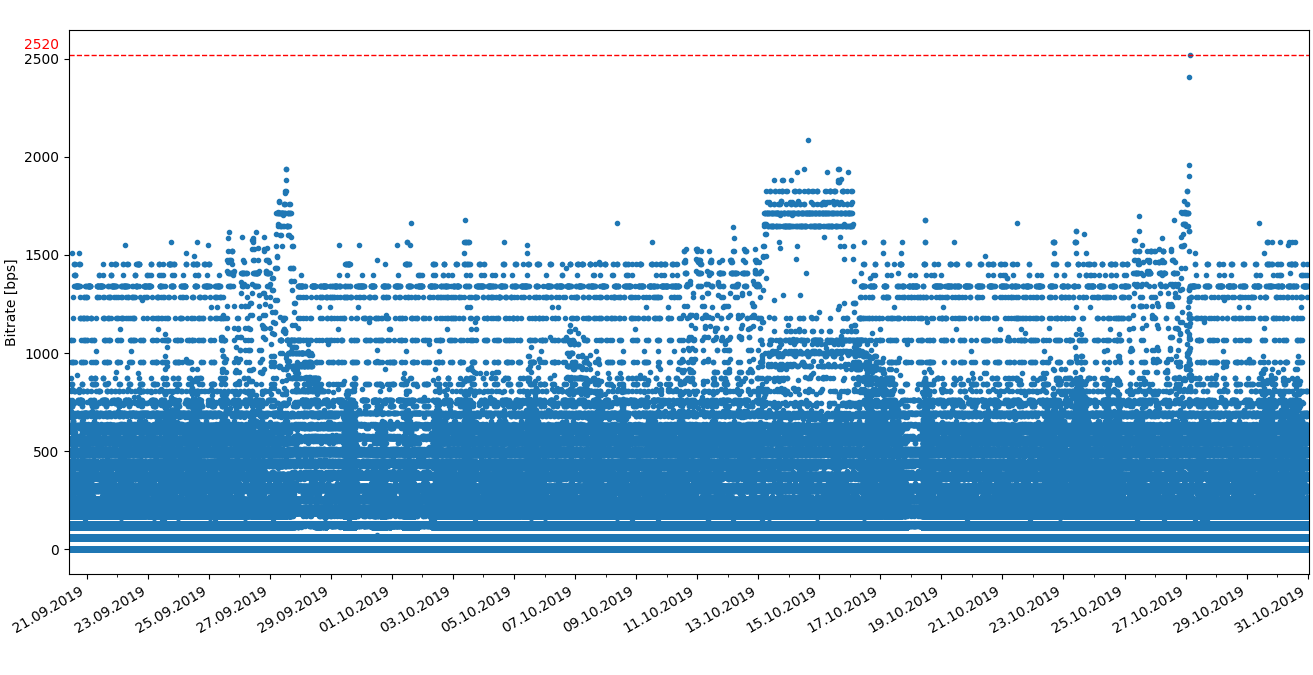
\includegraphics[width=1\textwidth]{03-dr-measured}
    \caption{Měřená rychlost přenosu dat [bps] v síti RS485 během doby testování}
    % \caption{Measured data rate in [bps] in RS485 network during long-term operation test}
    \label{fig:PacketLengthMeasuredAll}
\end{figure*}

Na základě frekvenční analýzy uvedené v tabulce \ref{tab:FreqAnalysis} a IMA know-how, pakety přenášející data z koncových zařízení jsou dlouhé 19 bytů a pakety potvrzení IMA protokolu jsou dlouhé 7 bytů. Alespoň dva pakety jsou potřeba k přenesení dat z koncových zařízení přes síť RS485, tj. paket s daty koncového zařízení a paket potvrzení.

V obrázku \ref{fig:PacketLengthMeasuredAll} jsou dvě důležité charakteristiky, maximální délka paketu 
(červená přerušovaná čára) a medián délky paketu (červená nepřerušovaná čára), určeny frekvenční analýzou v tabulce \ref{tab:FreqAnalysis}. 
Průměrné zatížení provozu kanálu sítě RS485 je 6,38 pps, tj. 0,85 Bps.
%shows lengths of captured packet  during
%Median of packet length is determined by using frequency analysis method, as shown in Tab. \ref{tab:FreqAnalysis}.
% 7,51 Byte --> simple arithmetic mean


Z testování provozu jsou zachyceny délky přenášených paketů ($ l $) s časovou přesností na tisícinu sekundy. Údaje o čase jsou převedeny na jednotky sekund pomocí funkce sum, aby byly získány data jako bitová rychlost v bitech za sekundu (bps),
V obrázku \ref{fig:PacketLengthMeasuredAll} červená přerušovaná čára s hodnotou 2520~bps) ukazuje jeden sekundový interval ve kterém součet přenesených paketů v síti RS485.
Na základě podrobných znalosti protokolu IMA se ukazuje, že je využito méně než 20\% kapacity sítě RS485 
%This limit state is caused by data communication of two sensor nodes that occupied 2\% of capacity of used RS485 network.

Aby bylo zabráněno přetížení sítě RS485, maximální počet koncových zařízení připojených ke gatewayi $ S_{MAX} $ je možné vypočítat vztahem:

\begin{equation}
S_{MAX} = \frac{\frac{\frac{v_{485}}{B}}{l_{MAX}} - R}{P}
\label{equ:max-count-of-sensors}
\end{equation}

kde:

\begin{tabular}{l @{  } l}
$v_{485}$ & rychlost přenosu dat v síti RS485 [bps]\\
 B        & počet bitů v bytu (pro přepočítání rychlosti přenosu dat na byty) \\
$l_{MAX}$ & maximální délka paketu \\
 R        & rezerva rychlosti přenosu dat [\%]\\
 P        & počt paketů k přenesení dat z koncového zařízení \\
\end{tabular}


S ohledem na výše uvedené limity, navržené rezervy a rychlosti přenosu dat v síti RS485 je vypočítán maximální počet koncových zařízení senzorové sítě, které souběžně odesílají data přes síť RS485 viz. tabulka \ref{tab:max-sensor-nodes}.

Použité hodnoty pro výpočet jsou:

\begin{tabular}{l @{ $=$ } l}
$v_{485}$ & RS485 network data rate \\
 B        & 8 \\
$l_{MAX}$ & 40 \\
 P        & 2 \\
\end{tabular}

\begin{table}[h]
\centering
\footnotesize
\caption{Maxímální počet připojených koncových zařízení v senzorové síti souběžně odesílající data skrze síť RS485 s určitou rezervou} 
\begin{ctucolortab}
\begin{tabular} {|p{2.5cm}|llll|}
    \hline

\textbf{RS485 rychlost přenosu dat} &       \multicolumn{4}{c|}{\textbf{Rezerva R}}	  	    \\

$v_{485}$ {[bps]}  &	0 \%	&	10 \%	&	20 \%	&	30 \%  \\ \hline

  1200~~~ &    1	&    1	&    1	&    1 \\
  2400~~~ &    3	&    3	&    3	&    2 \\
  4800~~~ &    7	&    6	&    6	&    5 \\
  9600~~~ &   15	&   13	&   12	&   10 \\
 19200~~~ &   30	&   27	&   24	&   21 \\
 38400~~~ &   60	&   54	&   48	&   42 \\
 57600~~~ &   90	&   81	&   72	&   63 \\
115200~~~ &  180	&  162	&  144	&  126 \\
230400~~~ &  360	&  324	&  288	&  252 \\
460800~~~ &  720	&  648	&  576	&  504 \\
921600~~~ & 1440	& 1296	& 1152	& 1008 \\
\hline

\end{tabular}
\end{ctucolortab}

\label{tab:max-sensor-nodes}
\end{table}


Např. v senzorové síti může být až 54 koncových zařízení připojených ke gatewayi, která je napojena na síť RS485 s přenosovou rychlostí 38400~bps a rezervou 10 \% nebo 42 koncových zařízení s přenosovou rychlostí 38400~bps a rezervou 30 \%.
Tento výsledek ukazuje, že jeden blok patra univerzity, tj. jedna síť RS485 je schopna fungovat s desítkami koncovými zařízeními senzorové sítě souběžně vysílající data s dostatečnou rezervou chránící přístupový systém. 






%%%%%%%%%%%%%%%%%%%%%%%%%%%%%%%%%%%%%%%%%%%%%%%%%%%%%%%%%%%%%%%%%%%%%%%%%%%%%%%%%%%%%%%
%       NOT USED
%%%%%%%%%%%%%%%%%%%%%%%%%%%%%%%%%%%%%%%%%%%%%%%%%%%%%%%%%%%%%%%%%%%%%%%%%%%%%%%%%%%%%%%
% The heavy traffic test simulates data transmission in the RS485 network as evidence of theoretically calculated values as shown in Tab \ref{tab:max-sensor-nodes}.

% \begin{figure}[!ht]
    % \centering
    % 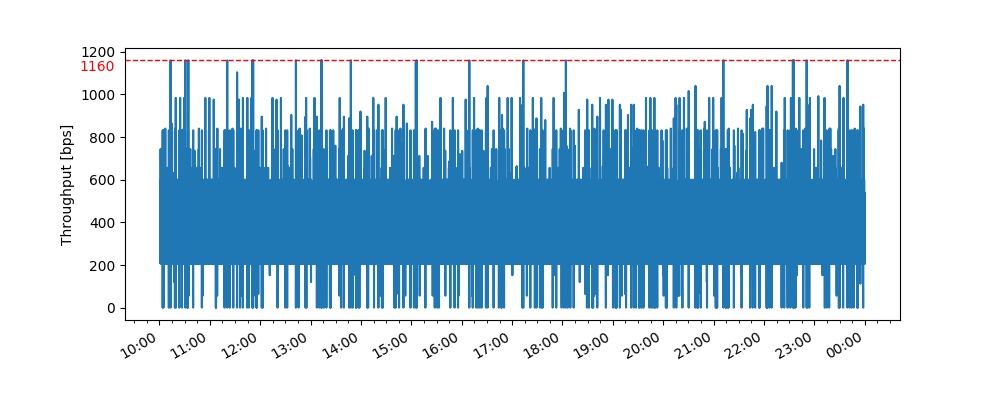
\includegraphics[width=.5\textwidth]{03-tp-simul}
    % \caption{RS485 datarates in simulation of heavy data traffic}
    % \label{fig:heavySimulation}
% \end{figure}

% This test simulated the transmission of more than 190~000 commands from 300 sensor nodes every 5 minutes simultaneously for 12 hours time period. The highest datarate achieved during simulation is 1160~bps, Fig \ref{fig:heavySimulation} red dashed line.

%!!! Tady to mozna chce frekvencni analyzu GW, at vis, jak jsou dlouhe pakety, pak nemusis hadat, nebo napis, ze max. delka je 19 bytů.

%Considering the worst case, ie packets with length of 40 Bytes, we have analytically calculated the maximum number of sensors a network can transmit based on the network transmission rate.

%\textbf{!!! Limit RS485: up to 32 transceivers on the serial bus !!! My vsak mame senzory pres LoRa ...Jo, ale to je fyzicky, to splnujeme, mame jich 13 :-)}
%datasheet: https://www.sparkfun.com/datasheets/Components/General/sp3485CN-LTR.pdf

%Space for peaks 10\% --> maximum packet rate is 324 pps
%Data measured in testing procedure shows Fig.

%\begin{table}[h]
%\centering
%\footnotesize
%\caption{Simple analytics of measured data}
%\begin{tabular}{lr}
%\textbf{Packet length} & \textbf{Bytes} \\ \hline
%Minimum   &   7 B     \\
%Maximum   &  40 B     \\
%mean      &   7,51 B  \\
%Median    &   7 B     \\
%\end{tabular}
%\label{tab: simple-analytics}
%\end{table}


%---
% tabulka, rezervy 10%, 30% ...
% Zjistit kolik sensoru muze byt na sbernici 485.
% popis os co  je co

\chapter{Návrh vylepšení systému}
V této kapitole jsou navrženy způsoby vylepšení navrženého systému.



Jedním z největších omezení navrženého systému je, že FW gatewaye musí podporovat typy všech koncových zařízení senzorové sítě.
Například použitý typ koncového zařízení RHF1S001






%%%%%%%%%%%%%%%%%%%%%%%%%%%%%%%%%%%%%%%%%%%%%%%%%%%%%%
\section{Návrh gatewaye verze 2}
Pro lepší mechanické uspořádání byla navržena verze 2 s navrženým plošným spojem (PCB).
Schéma zapojení je v obrázku \ref{fig:minigateway_schema} a plošný spoj je v obrázku \ref{fig:minigateway_plosnak}.
Je zde použit jiný vývojový kit NUCLEO-L432KC s výkonnějšim procesorem STM32L432KC, který má pinout stejný jako Arduino Nano, tedy je pod tímto názvem ve shcématu.
LoRa transceiver je použit RFM95w \cite{RFM95w} bez shieldu.
RS485 transceiver je použit LTC1480. 
Do zařízení je dále přidán externí stabilizátor, napěťový filtr, přepínač volitelné impedanční zakončení sítě RS485 a napěťové ochrany pro linky A, B a napájení. 

\begin{figure}[!h]
    \centering
    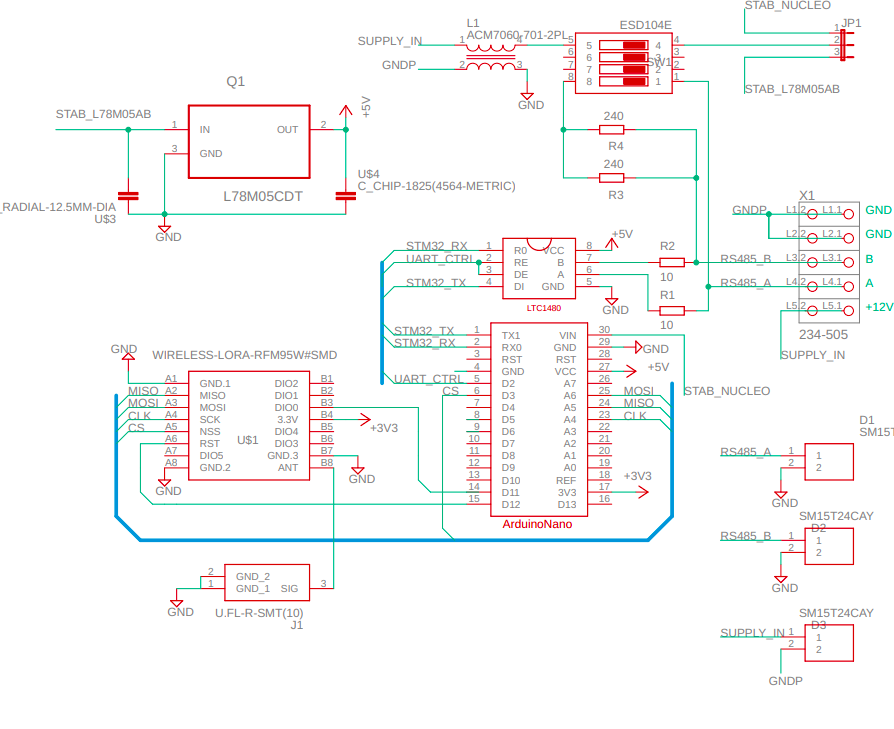
\includegraphics[width=1\textwidth]{minigateway_schema}
    \caption{Návrh gatewaye verze 2 - schéma}
    \label{fig:minigateway_schema}
\end{figure}

\begin{figure}[!h]
    \centering
    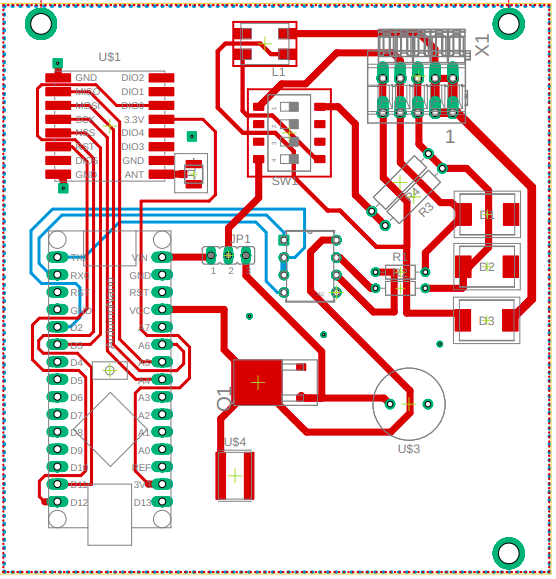
\includegraphics[width=0.7\textwidth]{minigateway_plosnak}
    \caption{Návrh gatewaye verze 2 - plošný spoj}
    \label{fig:minigateway_plosnak}
\end{figure}

Použitý procesor neobsahuje paměť EEPROM, tudíž pro ukládání konfigurace gatewaye a zařízení senzorové sítě je použita paměť flash.




\chapter{Závěr}
V této práci jsou diskutovány podmínky rozšíření stávajícího přístupového systému pracujícího s průmyslově standardizovanou sítí RS485 o bezdrátovou senzorovou síť založenou na LoRaWAN protokolu v jednokanálovém módu.
Dále je takováto senzorová síť navržena a realizována vytvořením prototypu jednokanálové LoRaWAN gatewaye připojené do sítě RS485 infrastruktury přístupového systému, kde jsou připojeny tzv. CKP zařízení ovládající dveřní zámky a čtečky, komunikující vlastním proprietárním CKP protokolem, který podoruje i navržená gateway.
K navržené gatewayi jsou připojeny LoRaWAN senzory třetích stran jako koncová zařízení senzorové sítě.
Na univerzitě, kde je tento přístupový systém zaveden, je proveden test dlouhodobého provozu. Při tomto testu je navržená gateway připojena do jedné sítě RS485, která již obsahje 12 CKP zařízení (páry čteček a dveřních zámků) a ke gatewayi jsou připojena dva LoRaWAN senzory jako koncová zařízení senzorové sítě.
Během doby testování jsou zaznamenávány přenášené pakety v síti RS485.
Ze zaznamenaných dat je provedena frekvenční analíza délek paketů, a je vypočítán maximální počet koncových zařízení senzorové sítě souběžně odesílajících data, v závislosti na rychlosti přenosu dat v síti RS485 a rezervě přenosové rychlosti, pro zachování správné funkce přístupového systému.
Např. do sítě RS485 s přenosovou rychlostí 38400 bps, s rezervou 20 \% je možné připojit navrženou gatewaye senzorové sítě a k ní připojit až 48 koncových zařízení, což je dostačující pro systémy bezdrátového měření.




% a je zvažována největší hodnota délky paketu, stejně jako rezerva rychlosti přenosu dat v síti RS485 za účelem ochrany správné funkcionality systému řízení přístupu.
% Frequency analysis of packet lengths is performed and the biggest value of packet length is considered as well as the reserve of the RS485 data rate in order to protect the access control system from malfunction. 

% Z nměřených dat je vypočítán maximální počet koncových zařízení senzorové sítě souběžně odesílajících data, v závislosti na rychlosti přenosu dat v síti RS485 a rezervě přenosové rychlosti, např 81 koncových zařízení připojených ke gatewayi senzorové sítě, napojené do sítě RS485 s přenosovou rychlostí 57600~bps a 10 \% rezervou. 
% This number of sensor nodes significantly exceeds the actual needs of the sensor nodes on one floor block of university building. Therefore we can state that WSN is suitable for smart metering applications.




%%%%%%%%%%%%%%%%%%%%%%%%%%%%%%%%%%%%%%%%%%%%%%%%
\bibliographystyle{amsalpha}
\bibliographystyle{csn690}
\bibliography{mybibliographyfile}
\begin{thebibliography}{9}
%%%%%%%%%%%%%%%%%%%%%%%%%%%%%%%%%%%%%%%%%%%%%%%%%%%%%%%%%%%%%%%



\bibitem[1]{nucleoST}
\textit{
NUCLEO-L073RZ.
}
ST Microelectronics
[Online]. Available:
\url{
https://www.st.com/en/evaluation-tools/nucleo-l073rz.html
}
[Accessed: 20-Sep-2019].

%___________________

\bibitem[2]{nucleoMbed}
\textit{
NUCLEO-L073RZ
}
ARM Mbed.
[Online]. Available:
\url{
https://os.mbed.com/platforms/ST-Nucleo-L073RZ/
}
[Accessed: 20-Sep-2019].

%___________________

\bibitem[3]{RFM95w}
\textit{
RFM95/96/97/98(W) - Low Power Long Range Transceiver Module}.
HopeRF electronic.
V1.0.
[Online]. Available:
\url{
http://wiki.dragino.com/index.php?title=Lora_Shield
}
[Accessed: 20-Sep-2019].

%___________________


\bibitem[4]{draginoWiki}
\textit{
Lora Shield.
}
Dragino.
[Online]. Available:
\url{
http://wiki.dragino.com/index.php?title=Lora_Shield
}
[Accessed: 20-Sep-2019].

%___________________


\bibitem[5]{AESlib}
\textit{
tiny-AES128-C
}
bitdust.
[Online]. Available:
\url{
https://github.com/bitdust/tiny-AES128-C
}
[Accessed: 20-Sep-2019].

%___________________


\bibitem[6]{CMAClib}
\textit{
openpana.
}
OpenPANA.
[Online]. Available:
\url{
https://github.com/OpenPANA/openpana
}
[Accessed: 20-Sep-2019].

%___________________


\bibitem[7]{rs485tr}
\textit{
SparkFun Transceiver Breakout - RS-485
}
Sparkfun.
[Online]. Available:
\url{
https://www.sparkfun.com/products/10124
}
[Accessed: 20-Sep-2019].


%___________________


\bibitem[8]{lwSpec}
\textit{
LoRaWAN Specification
}.
LoRa Alliance.
v1.1.
Sparkfun.
[Online]. Available:
\url{
https://lora-alliance.org/resource-hub/lorawantm-specification-v11
}
[Accessed: 20-Sep-2019].


%___________________


\bibitem[9]{lwSecur}
Robert Miller.
\textit{
LoRa Security
Building a Secure LoRa Solution.
}
MWR Labs Whitepaper.
[Online]. Available:
\url{
https://labs.mwrinfosecurity.com/assets/BlogFiles/mwri-LoRa-security-guide-1.2-2016-03-22.pdf
}
[Accessed: 20-Sep-2019].




% -------------------------
\bibitem[10]{accessControlSystem_eiprocus}
% \textit{

% }

[Online]. Available:
\url{
https://www.elprocus.com/understanding-about-types-of-access-control-systems/
}
[Accessed: 9-Sep-2019].


% -------------------------
\bibitem[11]{high density LPWAN}
% \textit{

% }

[Online]. Available:
\url{
https://ieeexplore.ieee.org/stamp/stamp.jsp?tp=&arnumber=8678997
}
[Accessed: 9-Sep-2019].

% -------------------------
\bibitem[12]{IoT cisco study}
% \textit{

% }

[Online]. Available:
\url{
https://blogs.cisco.com/innovation/the-internet-of-things-5-predictions-for-2018
}
[Accessed: 9-Sep-2019].

% % -------------------------
\bibitem[2]{IoT cisco study 02}
% \textit{

% }

[Online]. Available:
\url{
https://www.cisco.com/c/dam/en_us/about/ac79/docs/innov/IoT_IBSG_0411FINAL.pdf
}
[Accessed: 9-Sep-2019].

% % -------------------------
% \bibitem[2]{2}
% \textit{

% }

% [Online]. Available:
% \url{

% }
% [Accessed: 9-Sep-2019].

% % -------------------------
% \bibitem[2]{2}
% \textit{

% }

% [Online]. Available:
% \url{

% }
% [Accessed: 9-Sep-2019].

% % -------------------------
% \bibitem[2]{2}
% \textit{

% }

% [Online]. Available:
% \url{

% }
% [Accessed: 9-Sep-2019].

% % -------------------------
% \bibitem[2]{2}
% \textit{

% }

% [Online]. Available:
% \url{

% }
% [Accessed: 9-Sep-2019].





\end{thebibliography}

%\appendix


\end{document}ß